% This is samplepaper.tex, a sample chapter demonstrating the
% LLNCS macro package for Springer Computer Science proceedings;
% Version 2.20 of 2017/10/04
%
\documentclass[runningheads]{llncs}
%
\usepackage{graphicx,subfig}
\usepackage{amstext,amsmath,amssymb,bm,bbm,mathtools}
\usepackage[linesnumbered,lined,boxed,commentsnumbered]{algorithm2e}
\usepackage[export]{adjustbox}
\usepackage{xcolor}

\DeclareMathOperator*{\argmin}{arg\,min}
\DeclarePairedDelimiter\norm{\lVert}{\rVert}%
\DeclarePairedDelimiter\abs{\lvert}{\rvert}%

\newcommand{\todo}[1]{{\textcolor{blue}{#1}}}
\newcommand{\test}[1]{{\textcolor{red}{#1}}}
\newcommand{\jaco}[1]{{\textcolor{green!50!black}{#1}}}

% Used for displaying a sample figure. If possible, figure files should
% be included in EPS format.
%
% If you use the hyperref package, please uncomment the following line
% to display URLs in blue roman font according to Springer's eBook style:
% \renewcommand\UrlFont{\color{blue}\rmfamily}

\begin{document}
%
\title{\jaco{A Digital Evolution Model for Image Segmentation guided by Elastica Energy}\thanks{This  work has  been  partially  funded by CoMeDiC ANR-15-CE40-0006 research grant.}}
%\title{Digital Curvature Evolution Models for Image Segmentation\thanks{This  work has  been  partially  funded by CoMeDiC ANR-15-CE40-0006 research grant.}}

\author{Daniel Antunes\inst{1}
Jacques-Olivier Lachaud\inst{1}
Hugues Talbot\inst{2}}
%
\authorrunning{D. Antunes et al.}
% First names are abbreviated in the running head.
% If there are more than two authors, 'et al.' is used.
%
\institute{Universit{\'e} Savoie Mont Blanc, LAMA, UMR CNRS 5127, F-73376, France
\email{daniel.martins-antunes, jacques-olivier.lachaud@univ-savoie.fr} \and
CentraleSupelec Inria \'equipe OPIS, Universit\'e Paris-Saclay, 9 rue Joliot-Curie, F-91190 Gif-sur-Yvette \\
\email{hugues.talbot@centralesupelec.fr}}
%
\maketitle              % typeset the header of the contribution
%
\begin{abstract}

 
\keywords{Multigrid convergence  \and Digital estimator \and Curvature \and Shape Optimization \and Image Segmentation.}
\end{abstract}
%
%
%
\setcounter{footnote}{0}
\section{Introduction \todo{(To be extended)}}


Geometric quantities are particularly useful as regularizers in
low-level image analysis, especially when little prior information is
known about the shape of interest. Length penalization is a general
purpose regularizer and the literature is vast on models that make use
of it, from active contours \cite{casseles97geodesic} to level-set
formulations \cite{malladi1995image,malladi1995shape}. Discrete
graph-based variational models have been particularly succesfull to
incorporate length penalization as a penalizer, while keeping the
ability to extract global optimum
\cite{boykov01graphcut,appleton05geodesic}.

However length regularization shows its limitations when segmenting
small or thin and elongated objects, as it tends to shrink solutions
or return disconnected solutions. Such drawbacks can be problematic in
image segmentation or image inpainting. It is thus rather natural to
consider curvature (especially squared curvature) has a potential
regularizer. Energies involving squared curvature are often called
{\em Euler elastica} model (it dates back to Euler) or {\em Willmore energy}
($n$-dimensional extension) and have been brought back to attention in
computer vision by Mumford \cite{mumford1994elastica}. A similar
regularizer is arguably also present in the second-order regularizer
of the famous snake model \cite{kass1988snakes}.

One of the first successful uses of curvature in image processing is
the inpainting algorithm described in \cite{masnou98inpainting}. The
authors evaluate the elastica energy along the level lines of a
simply-connected image to reconstruct its occluded parts. The
non-intersection property of level lines allows the construction of an
efficient dynamic programming algorithm. But one should keep in mind
that the curvature energy is very coarsely approximated. We may quote
\cite{chan02elasticainpainting} as another geometric inpainting method
involving elastica.

In image segmentation, Zehiry and Grady have shown that injecting
curvature as a regularizer allow to recover thin and elongated objects
\cite{zehiry10fast}. Similarly Schoenemann {\em et al.}
\cite{schoenemann09linear} have considered the elastica energy in
their ratio-based image segmentation approach. Their global
optimization framework shows the considerable interest of using such
regularizer in common binary image segmentation tasks. However the
time complexity of their algorithm is quite prohibitive, even if
curvature is rather coarsely approximated. 

In fact, it is still a very challenging task to inject curvature in
the context of image segmentation with global optimization.  The
state-of-art methods are difficult to optimize and not scalable
\cite{zehiry10fast,schoenemann09linear,strandmark11globalframework,nieuwenhuis14efficient}. In
order to achieve reasonable running times, such approaches make use of
coarse curvature estimations for which the approximation error is
unknown. Improving the quality of the curvature estimator has an
important impact on the accuracy of the results, but is
computationally too costly in these methods.

Segmentation methods using elastica or Willmore energies are generally
just computing the corresponding flow, i.e. following its
gradient. Well-founded level-set methods involving Willmore energy
\cite{droske2004level} have been used in medical image segmentation
\cite{lim2012introducing}. Another level-set formulation similar to
the Chan-Vese model has been proposed in \cite{zhu2013image}. Willmore
flow can also be carried out by phase-field models (see
\cite{bretin2015phase}) but they are less suited to image segmentation
since interfaces are blurred in such models. Threshold dynamics can
also be considered for such energies \cite{esedoglu2008threshold} and
has been proposed for image desocclusion \cite{esedoglu2005threshold}.

In this paper we are interested in purely discrete variational
segmentation models involving an elastica energy. As said above,
current methods use coarse approximation of curvatures in their
formulation.  Recently, new estimators of curvature along digital
contours have been proposed
\cite{roussillon11mdca,coeurjolly13integral,schindele17mdca} with the
remarkable multigrid convergence property. This motivates us to search
for models in which they can be used successfully.

We therefore investigate the use of the digital integral invariant
curvature estimator \cite{coeurjolly13integral} in a discrete
variational segmentation framework. More precisely, we show how to
incorporate it in a digital flow minimizing its squared
curvature. This model is expressible as a discrete combinatorial
optimization model, which we solve using a classical variant of QPBO
algorithm \cite{rother07qpbo}. We are not yet able to compute a global
solution to the whole domain, but our approach leads to a digital flow
similar to continuous Elasticas, as shown by our experiments. We
present an application of the model as a post-processing step in a
segmentation framework, and demonstrate how it can improve standard
results. The code is freely available on
github\footnote{https://www.github.com/danoan/BTools}.

%% In this work, we investigate the use of a more suitable curvature
%% estimator with multigrid convergent property and its application as a
%% boundary regularizer in a digital flow minimizing its squared
%% curvature. Our method decreases the elastica energy of the contour and
%% its evolution is evaluated on several digital flows.

%% Finally, we
%% present an application of the model as a post-processing step in a
%% segmentation framework. The code is freely available on
%% github\footnote{https://www.github.com/danoan/BTools}.


\begin{itemize}
\item{Geometric properties and regularization}
\item{The role of curvature} 
  
  Quote \cite{schoenemann2011elastic} for the interest of using curvature energy when segmenting regions in gradient-based data fitting term. It can look for global optimum within a graph representation of the image. Main problem of their approach is the computational complexity as well as rather coarse approximations of curvature. (Be more precise here).
  
\item{What are the difficulties in use curvatue as a regularizer (point out convex relaxation approaches) and how a digital approach may help us }
\item{Outline: We present two models that illustrate how digital estimators can be used to minimize the elastica energy on digital sets.  }
\item{\todo{Add related works : geometric priors, binary segmentation, other digital curve evolution models}}
\item{\todo{Talk about Willmore flow with phase field or with threshold dynamics}}
  
\item{\textbf{Classical work on elastica and Wilmore flow in imaging}}
  \begin{itemize}
  \item{Level lines based disocclusion \cite{masnou98inpainting} }	
  \item{Filling-In by Joint Interpolation of Vector Fields and Gray Levels \cite{ballester01filljoint} }
  \item{Eulers Elastica and Curvature Based Inpaintings \cite{chan02elasticainpainting} }
  \item{Discrete willmore flow \cite{bobenko2005discrete}}
  \item{Introducing Willmore flow into level set segmentation of spinal vertebrae \cite{lim2012introducing}}	
  \end{itemize}
  
\item{\textbf{Level-sets}}
  \begin{itemize}
  \item{Image processing via level set curvature flow \cite{malladi1995image} }
  \item{Shape Modeling with Front Propagation: A Level Set Approach \cite{malladi1995shape} }	
	\end{itemize}	
  
\item{\textbf{Convex relaxation}}
  \begin{itemize}
  \item{A convex lower semicontinuous approximation of Eulers elastica energy \cite{bredies15convex}}				\item{Introducing Total Curvature for Image Processing \cite{goldluecke11totalcurvature}}
  \end{itemize}	
  
\item{\textbf{Constraint optimization}}
  \begin{itemize}
  \item{Curvature regularity for region-based image segmentation and inpainting: A linear programming relaxation \cite{schoenemann09linear} }	
  \item{A Fast Algorithm for Euler's Elastica Model Using Augmented Lagrangian Method \cite{tai11elastica} }		
  \item{The elastic ratio: Introducing curvature into ratio-based image segmentation \cite{schoenemann2011elastic} }		
  \item{Curvature Regularization for Curves and Surfaces in a Global Optimization Framework \cite{strandmark11globalframework} }
  \end{itemize}
  
\item{\textbf{Discrete approaches}}
  \begin{itemize}
  \item{Fast global optimization of curvature \cite{zehiry10fast}	}
  \item{Efficient Squared Curvature \cite{nieuwenhuis14efficient} 	}
  \item{Contrast driven {E}lastica for image segmentation \cite{el2016contrast} }	
  \end{itemize}
  
	
\end{itemize}


\textit{Outline}. Section two reviews the concept of multigrid
convergence and highlights its importance for the definition of
digital estimators. Next, we describe two convergent estimators used
in this paper, one for tangent and the other for curvature. They are
used in the optimization model and in the definition of the digital
elastica. Section three describes the proposed curvature evolution
model along with several illustrations of digital flows. Section four
explains how to use the evolution model as a post-processing step in
an image segmentation framework. Finally, sections five and six
discuss the results and point directions for future work.



\section{Multigrid convergent estimators \todo{(Mostly copy/paste)}}
The goal of this section is to  introduce the concept of multigrid convergent and its interest in the analysis of digital images.
\begin{itemize}
	\item{Why to use multigrid convergent estimators}
	\item{Multigrid convergence for local estimators}
	\item{Reference to examples of multigrid digital estimators(for curvature, length, tangent)}
	\item{Define the elastica energy estimator}
	\item{\test{(Jaco) see if two opposite II evaluations give convergent curvature}}
\end{itemize}

\hrulefill

A digital image is the result of some quantization process over an object $X$ lying in some continuous space of
dimension $2$ (here).  For example, the Gauss digitization of $X$ with grid step $h>0$ is defined as
\begin{align*}
	D_h(X) = X \cap (h\mathbb{Z})^2.
\end{align*} 

Given an object $X$ and its digitization $D_h(X)$, a digital estimator $\hat{u}$ for some geometric quantity $u$ is
intended to compute $u(X)$ by using only the digitization. This problem is not well-posed, as the same digital object
could be the digitization of infinitely many objects very different from $X$. Therefore, a characterization of what constitutes
a good estimator is necessary.

Let $u$ be some geometric quantity of $X$ (e.g. tangent, curvature). We wish to devise a digital estimator $\hat{u}$ for
$u$. It is reasonable to state that $\hat{u}$ is a good estimator if $\hat{u}(D_h(X))$ converges to $u(X)$ as we refine
our grid. For example, counting pixels is a convergent estimator for area (with a rescale of $h^2$); but counting
boundary pixels (with a rescale of $h$) is not a convergent estimator for perimeter. Multigrid convergence is the
mathematical tool that makes this definition precise. Given any subset $Z$ of $(h\mathbb{Z})^2$, we can represent it as a
union of axis-aligned squares with edge length $h$ centered on the point of $Z$. The topological boundary of this union
of cubes is called {\em $h$-frontier} of $Z$. When $Z=D_h(X)$, we call it {\em $h$-boundary of $X$} and denote it by
$\partial_h X$.
%% In the following, let the $h$-frontier of $D_h(X)$ to be defined as $\partial D_h(X) = \partial \left( \frac{1}{h} \cdot X \right) \cap \mathbb{Z}^2$.

\begin{definition}[Multigrid convergence for local geometric quantites]
  A local discrete geometric estimator $\hat{u}$ of some geometric
  quantity $u$ is (uniformly) multigrid convergent for the family $\mathbb{X}$ if
  and only if, for any $X \in \mathbb{X}$, there exists a grid step
  $h_X>0$ such that the estimate $\hat{u}(D_h(X),\hat{x},h)$ is
  defined for all $\hat{x} \in \partial_hX$ with $ 0 < h < h_X$, and
  for any $x \in \partial X$,
  \begin{equation*}
    \forall \hat{x} \in  \partial_hX \text{ with } \norm{ \hat{x} - x }_{\infty} \leq h, \norm{ \hat{u}(D_h(X),\hat{x},h) - u(X,x)} \leq \tau_{X}(h),			
  \end{equation*}
  where $\tau_{X}:\mathbb{R}^{+}\setminus\{0\} \rightarrow
  \mathbb{R}^{+}$ has null limit at $0$. This function defines the
  speed of convergence of $\hat{u}$ towards $u$ for $X$.
\end{definition}
	
For a global geometric quantity (e.g. perimeter, area, volume), the definition remains the same, except that the mapping
between $\partial X$ and $\partial_h X$ is no longer necessary.
	
Multigrid convergent estimators provide a quality guaranty and should be preferred over non-multigrid convergent
ones. In the next section, we describe two estimators that are important for our purpose.

\subsection{Tangent and Perimeter Estimators}

The literature presents several perimeter estimators that are multigrid convergent (see
\cite{coeurjolly04comparative,coeurjolly12multigrid} for a review), but in order to define the digital elastica we need a local estimation
of length and we wish that integration over these local length elements gives a multigrid convergent estimator for the
perimeter.

\begin{definition}[Elementary Length]
  Let a digital curve $C$ be represented as a sequence of grid vertices in a grid cell representation of digital objects (in grid with step $h$). Further, let $\vec{ \hat{v} }$ be a multigrid convergent estimator for the tangent vector. The elementary length $\hat{s}(\vec{e})$ at some oriented grid edge $ \vec{e} \in C$ is defined as
  \begin{align*}
    \hat{s}(\vec{e}) = h \cdot \vec{\hat{v}}(\vec{e}) \cdot \vec{e}.
  \end{align*}
\end{definition}
The integration of the elementary length along the digital curve is a multigrid convergent estimator for perimeter if
one uses the $\lambda$-MST \cite{lachaud07tangent} tangent estimator (see \cite{lachaud06hdr}).

\subsection{Integral Invariant Curvature Estimator}
Generally, an invariant $\sigma$ is a real-valued function from some space $\Omega$ which value is unaffected by the action
of some group $\mathfrak{G}$ on the elements of the domain
\begin{align*}
  x \in \Omega, g \in \mathfrak{G}, \sigma(x) = v \longleftrightarrow \sigma(g \cdot x ) = v.
\end{align*}
Perimeter and curvature are examples of invariants for shapes on $\mathbb{R}^2$ with respect to the euclidean group
(rigid transformations). Definition of integral area invariant and its one-to-one correspondence with curvature is
proven in \cite{manay04intinvariant}.


\begin{definition}[Integral area invariant]
  Let $X \subset \mathbb{R}^2$ and $B_r(p)$ the ball of radius $r$ centered at point $p$. Further, let
  $\mathbbm{1}_X(\cdot)$ be the characteristic function of $X$. The integral area invariant $\sigma_{X,r}(\cdot)$ is
  defined as
  \begin{align*}
    \forall p \in \partial X, \quad \sigma_{X,r}(p) = \int_{B_r(p)}{ \mathbbm{1}_X(x) dx}.
  \end{align*}
\end{definition}


The value $\sigma_{X,r}(p)$ is the intersection area of ball $B_r(p)$ with shape $X$. By locally approximating the shape
at point $p \in X$, one can rewrite the intersection area $\sigma_{X,r}(p)$ in the form of the Taylor expansion
\cite{pottman09intinvariant}
	
\begin{align*}
  \sigma_{X,r}(p) = \frac{\pi}{2}r^2 - \frac{\kappa(X,p)}{3}r^3 + O(r^4),
\end{align*}
		
where $\kappa(X,p)$ is the curvature of $X$ at point $p$. By isolating $\kappa$ we can define a curvature estimator
	
\begin{align}
  \tilde{\kappa}(p) \coloneqq \frac{3}{r^3}\left( \frac{\pi r^2}{2} - \sigma_{X,r}(p) \right),
  \label{eq:curvature_approximation}
\end{align}
	
Such an approximation is convenient as one can simply devise a multigrid convergent estimator for the area.

\begin{definition}	
  Given a digital shape $D \subset (h \mathbb{Z})^2$, a multigrid convergent estimator for the area $\widehat{Area}(D,h)$ is defined as	
		
  \begin{align}
    \widehat{Area}(D,h) \coloneqq h^2\text{Card}\left( D \right).	
    \label{eq:digital_estimator_area}
  \end{align}
\end{definition}
	
In \cite{coeurjolly13integral}, the authors combine the approximation\eqref{eq:curvature_approximation} and digital estimator
\eqref{eq:digital_estimator_area} to define a multigrid convergent estimator for the curvature.

\begin{definition}[Integral Invariant Curvature Estimator]
  Let $D \subset (h \mathbb{Z})^2$ a digital shape. The integral invariant curvature estimator is defined as
  \begin{align*}
    \hat{\kappa}_{r}(D,x,h) \coloneqq \frac{3}{r^3} \left( \frac{\pi r^2}{2} - \widehat{Area} \left( B_{r} ( x ) \cap D, h \right) \right).
    %% \hat{\kappa}_{r}(D,x,h) \coloneqq \frac{3}{r^3} \left( \frac{\pi r^2}{2} - \widehat{Area} \left( B_{r/h} ( \frac{1}{h} \cdot x ) \cap D, h \right) \right).
  \end{align*}
\end{definition}


This estimator is robust to noise and can be extended to estimate the mean curvature of three dimensional shapes.

\subsection{Elastica energy estimator}

In the remaining of this paper we are going to be interested in the minimization of the elastica energy. Given an euclidean shape $X$, the elastica is defined as

\begin{align}
  E(X) = \int_{\partial X}{(\alpha + \beta \kappa^2) ds}, \quad \text{for~} \alpha \ge 0, \beta \ge 0.
  \label{eq:elastica}
\end{align}

We are going to use the digital version of the energy, using multigrid convergent estimators. The energy, in this case, is also multigrid convergent.


\begin{align}
	\hat{E}( D_h(X) ) = \sum_{x \in \partial D_h(X)}{ \hat{s}(x)\left(\; \alpha + \beta \hat{\kappa}_{r}^2(D_h(X),x,h) \; \right)}.
	\label{eq:digital-energy}
\end{align}
 In the following we omit the grid step $h$ to simplify expressions (or, putting it differently, we assume that $X$ is rescaled by $1/h$ and we set $h=1$).

\section{Local combinatorial optimization}

The objectives of this section is to show both the potential of minimizing a purely digital Elastica energy but also to underline the difficulties of using it in a global combinatorial optimization framework.

Given a digital shape $S^{(0)}$ we describe a process that generates a sequence $S^{(i)}$ of shapes with non-increasing
elastica energy. The idea is to define a neighborhood of shapes
$\mathcal{N}^{(i)}$ to the shape $S^{(i)}$ and choose the element of
$\mathcal{N}^{(i)}$ with lowest energy.  The process is suited for the
integral invariant estimator but also for other curvature estimators,
for example, MDCA \cite{roussillon11mdca}.

Let $S$ be a $2$-dimensional digital shape. We adopt the cellular-grid model to represent $S$, i.e., pixels and its lower dimensional counterparts, linels and pointels, are part of $S$. In particular, we denote by $\partial S$ the topological boundary of $S$, i.e., the connected sequence of linels such that for each linel we have one of its incident pixels in $S$ and the other not in $S$.


Let $d_{S}:\Omega \rightarrow \mathcal{R}$ be the euclidean distance transformation with respect to shape $S$. The value $d_S(x)$ gives the euclidean distance between $x$ and the closest pixel in $S$. 

\begin{definition}[m-Ring Set]
Given a digital shape $S\in\Omega$, its distance transformation $d_S$ and natural numbers $m,r > 0$, we define its $m$-ring set as

\begin{align*}
	\quad R_m(S) &= R_m^-(S) \; \cup \; R_m^+(S) \\
	&= \left\{ x \in \Omega \; | \; m-1 < d_S(x) \leq m \right\} \; \cup \;  \left\{ x \in \Omega \; | \; 	m-1 < d_{\overline{S}}(x) \leq m \right\}\\
\end{align*}

\end{definition}

Consider the following set of neighbor candidates to $S$:

\begin{align*}
\mathcal{U}(S) = \{ D \; | D \subset R_1(S) \cup S \; \text{and} \; \text{$D$ is connected}. \}
\end{align*}


Such set can be extremely large and its complete exhaustion is prohibitively expensive.  Instead, we explore a subset of it with the help of $n$-glued curves.

An oriented closed curve $C$ is a sequence of linels. A segment of $C$ is a subsequence $c \in C$ of its linels.

\begin{figure}
\center
	\subfloat[\label{}]{%
	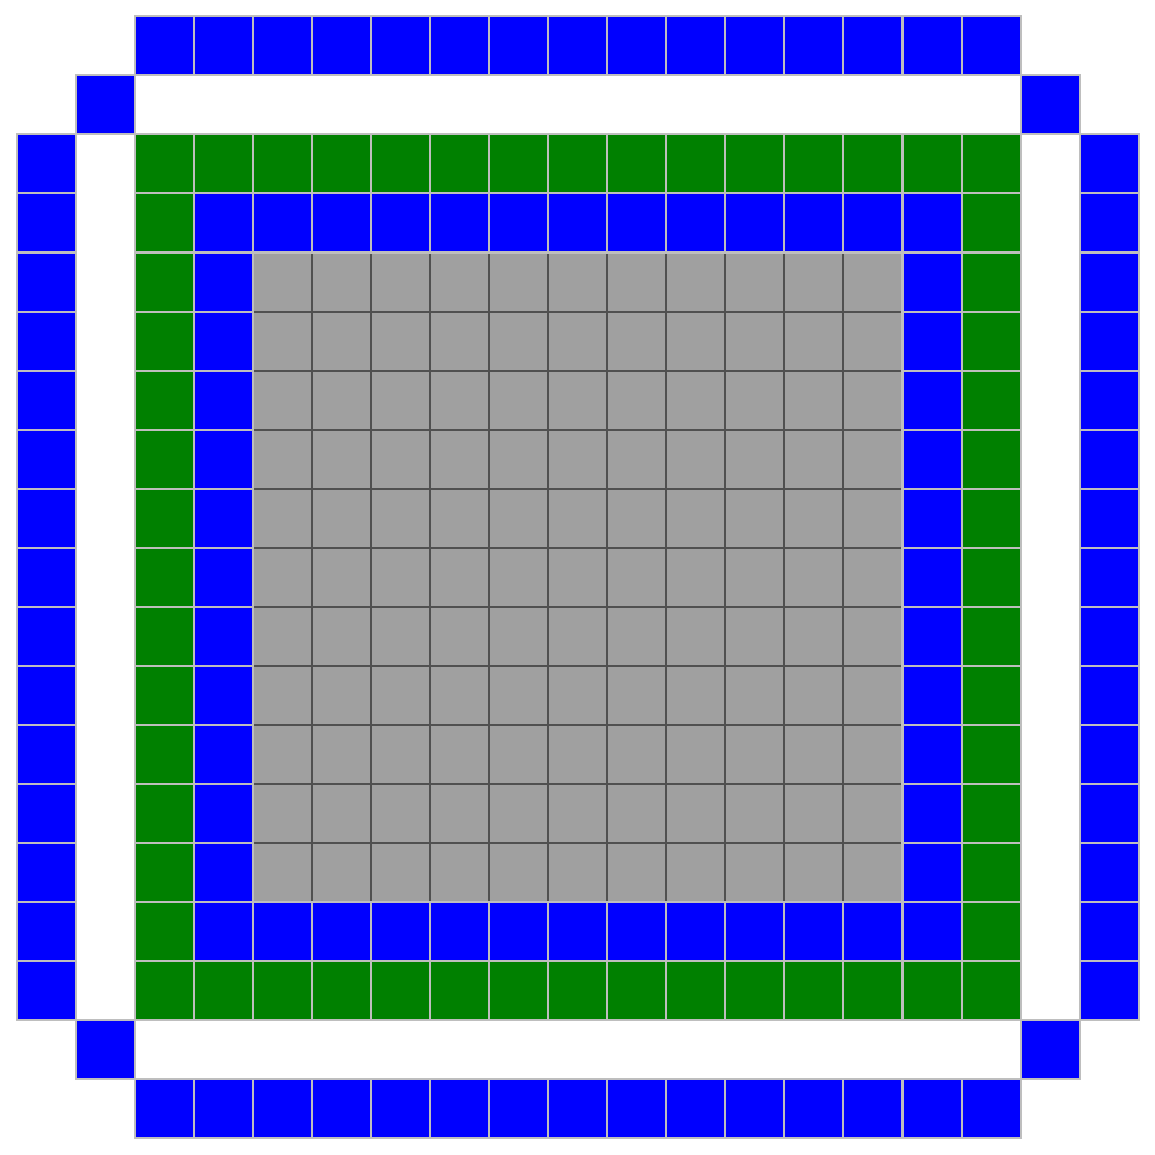
\includegraphics[scale=0.2]{images/local_search/definitions/model-regions-square.eps}
	}\hspace{40pt}%
	\subfloat[\label{}]{%
	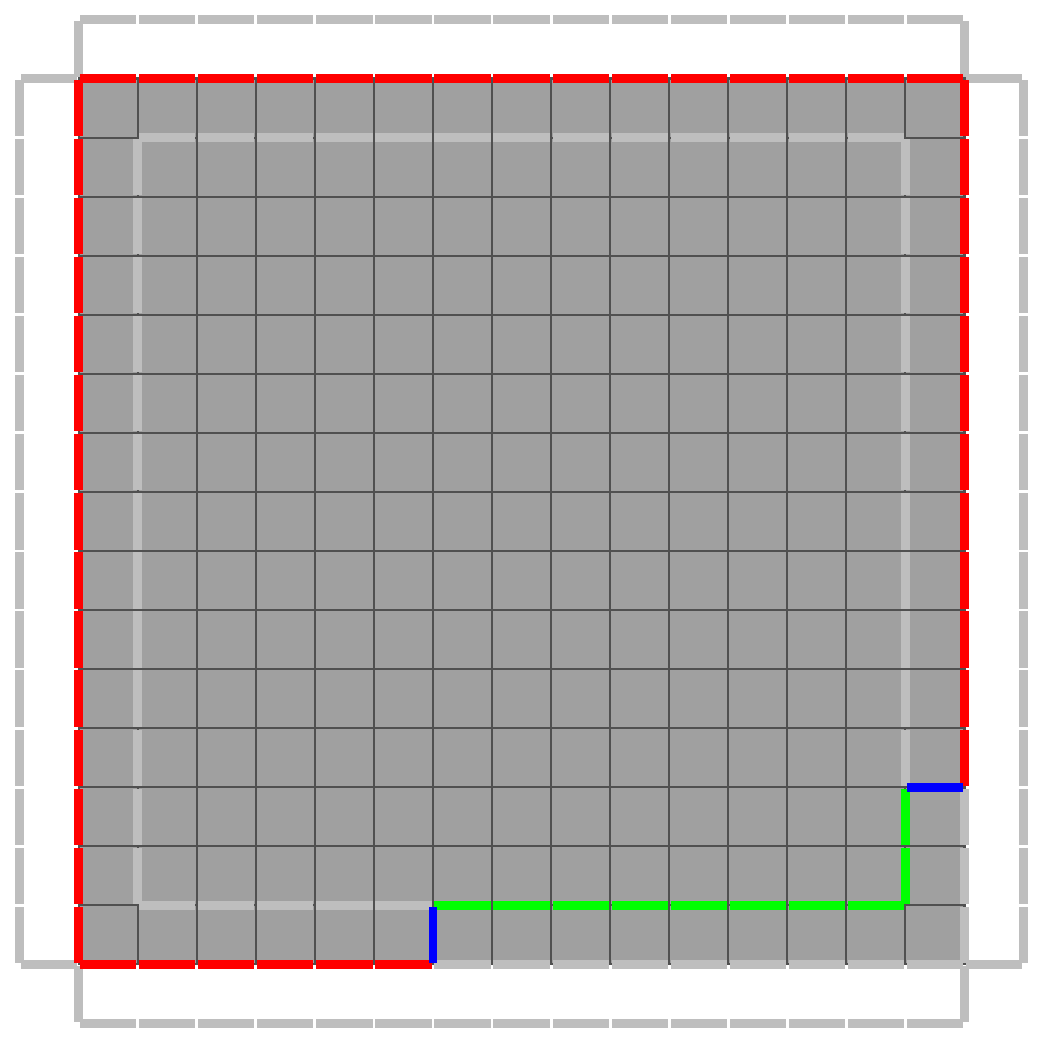
\includegraphics[scale=0.2]{images/local_search/definitions/glued-curve.eps}
	}%	
	\caption{The blue pixels in figure (a) illustrates a $2$-ring set, while the green pixels its inner-pixel boundary. In figure (b) we highlight an element of set $\mathcal{G}_{11}(C_1,C_2)$. The curve segments of $C_1$ and $C_2$ are colored in red and green, while the junction linels in blue.}
\end{figure}

\begin{definition}[Glued Curve]
Given closed curves $C_1,C_2$ agreeing with some orientation $q$, a glued curve is a closed curve  $(c_1,\ell_1,c_2,\ell_2)$ with orientation $q$ and $c_1 \in C_1, c_2 \in C_2$. The linels $\ell_1,\ell_2$ are called junction linels.
\end{definition}

\begin{definition}[$n$-Glued Curve Set]
Given closed curves $C_1,C_2$ with same orientation, its set of $n$-glued curves is defined as

\begin{align*}
	\mathcal{G}_n(C_1,C_2) = \{ (c_1,\ell_1,c_2,\ell_2) \; | \; |c_2|=n \},
\end{align*}
\end{definition}

Let $S_O = \partial ( S \setminus R_1^-(S) ) $ and $S_I = \partial ( S \cup R_1^+(S) )$, the neighborhood set to shape $S$ is defined as

\begin{align*}
	\mathcal{N}(S,N) = \bigcup_{1 \leq n \leq N} int \big( \; \mathcal{G}_{n}(\partial S, S_I) \;\big) \cup int \big( \; \mathcal{G}_{n}(\partial S, S_O) \; \big),
\end{align*}

where $int(C)$ is the interior of the shape bounded by oriented curve $C$. Algorithm~\ref{alg:local-search} describes the local combinatorial process and Figure~\ref{fig:local-comb-square-results} presents the digital curve evolution when executing this algorithm for two different shapes with $N=20$.


\begin{algorithm}
 \SetKwData{It}{i}
 \SetKwData{MIt}{maxIt}
 \SetKwData{Tol}{tolerance}
 \SetKwData{Delta}{delta}
 \SetKwData{Best}{best} 
 \SetKwInOut{Input}{input}\SetKwInOut{Output}{output}
 
 \Input{A digital set $S$; the maximum length of glued curves $N$; the maximum number of iterations \MIt; and a stop condition \Tol}
 \BlankLine
 \Delta $\longleftarrow$ \Tol+1\;
 \While{ \It $<$ \MIt \bf{and} \Delta $>$ \Tol  }{
  	\For{$ X \in \mathcal{N}(S^{(i)},N) $}
	{
		\If{ $\hat{E}(X)$ $<$ $\hat{E}(X^\star)$ }
		{
			$X^\star \longleftarrow X$
		}
	}
	\It $\longleftarrow$ \It $+1$\;
	$S^{(i)} \longleftarrow X^\star$\;
	\Delta $\longleftarrow$ $\hat{E}(S^{(i-1)}) - \hat{E}(S^{(i)})$\;	
 }
 \label{alg:local-search} 
 \caption{Local combinatorial optimization for elastica minimization.}
\end{algorithm}

		
\begin{figure}[!ht]
\center
	\subfloat[\label{}]{%
	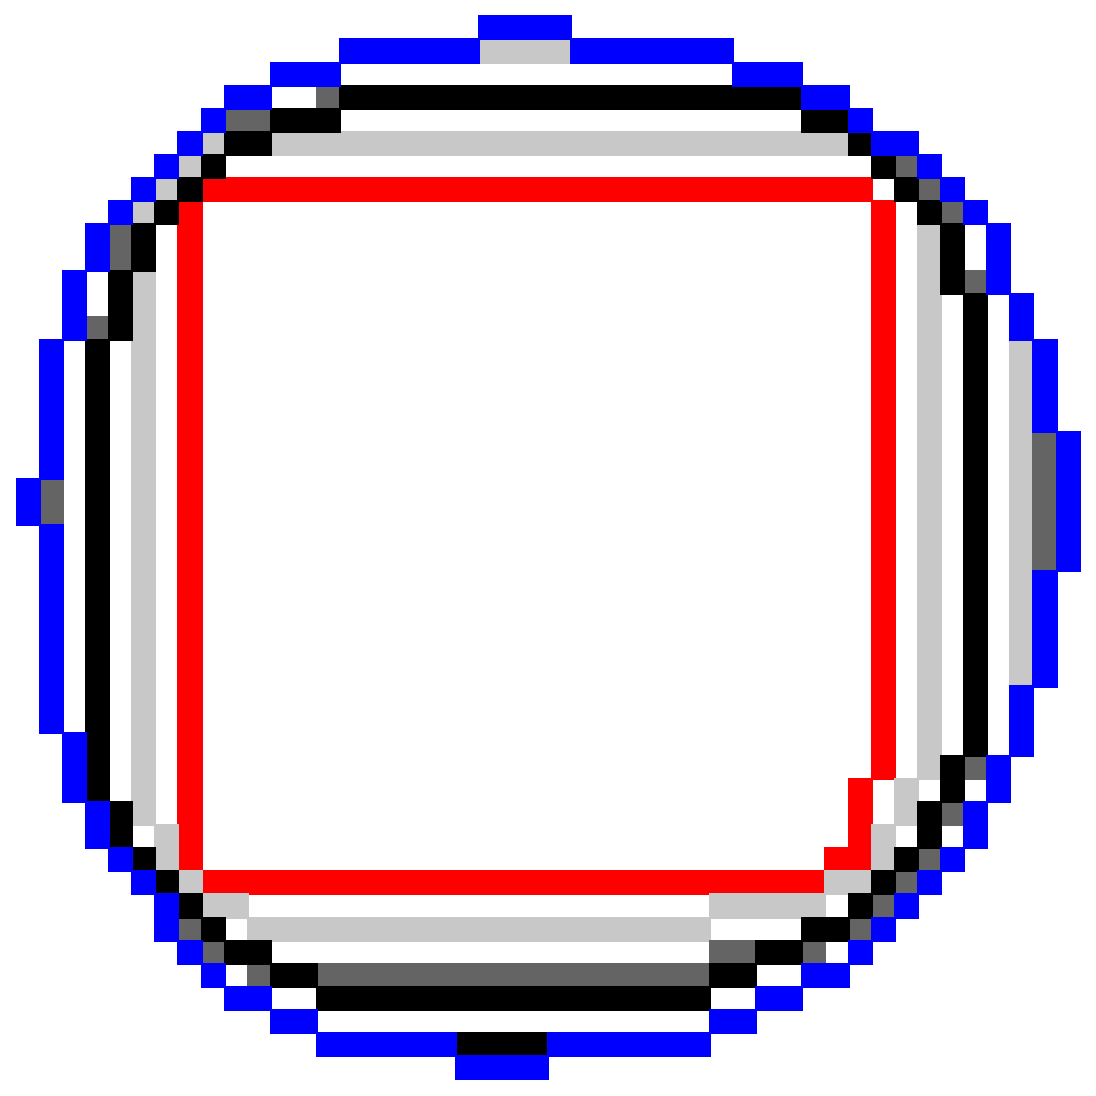
\includegraphics[scale=0.125]{images/local_search/square/h1.0/summary_flow.eps}
	}%
	\hspace{10pt}
	\subfloat[\label{}]{%
	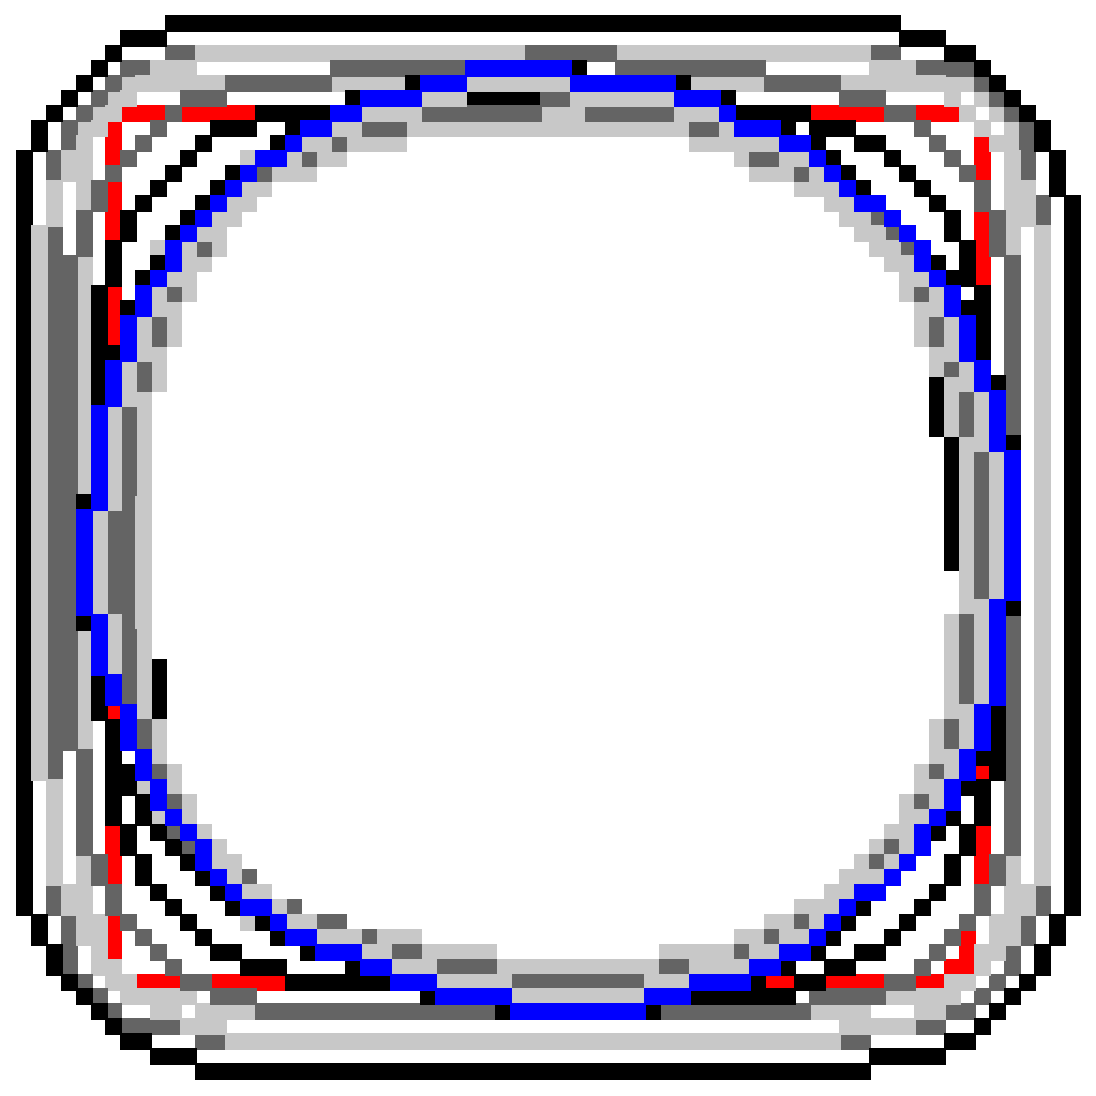
\includegraphics[scale=0.125]{images/local_search/square/h0.5/summary_flow.eps}
	}%
	\hspace{10pt}
	\subfloat[\label{}]{%
		\textbf{Missing figure}
	%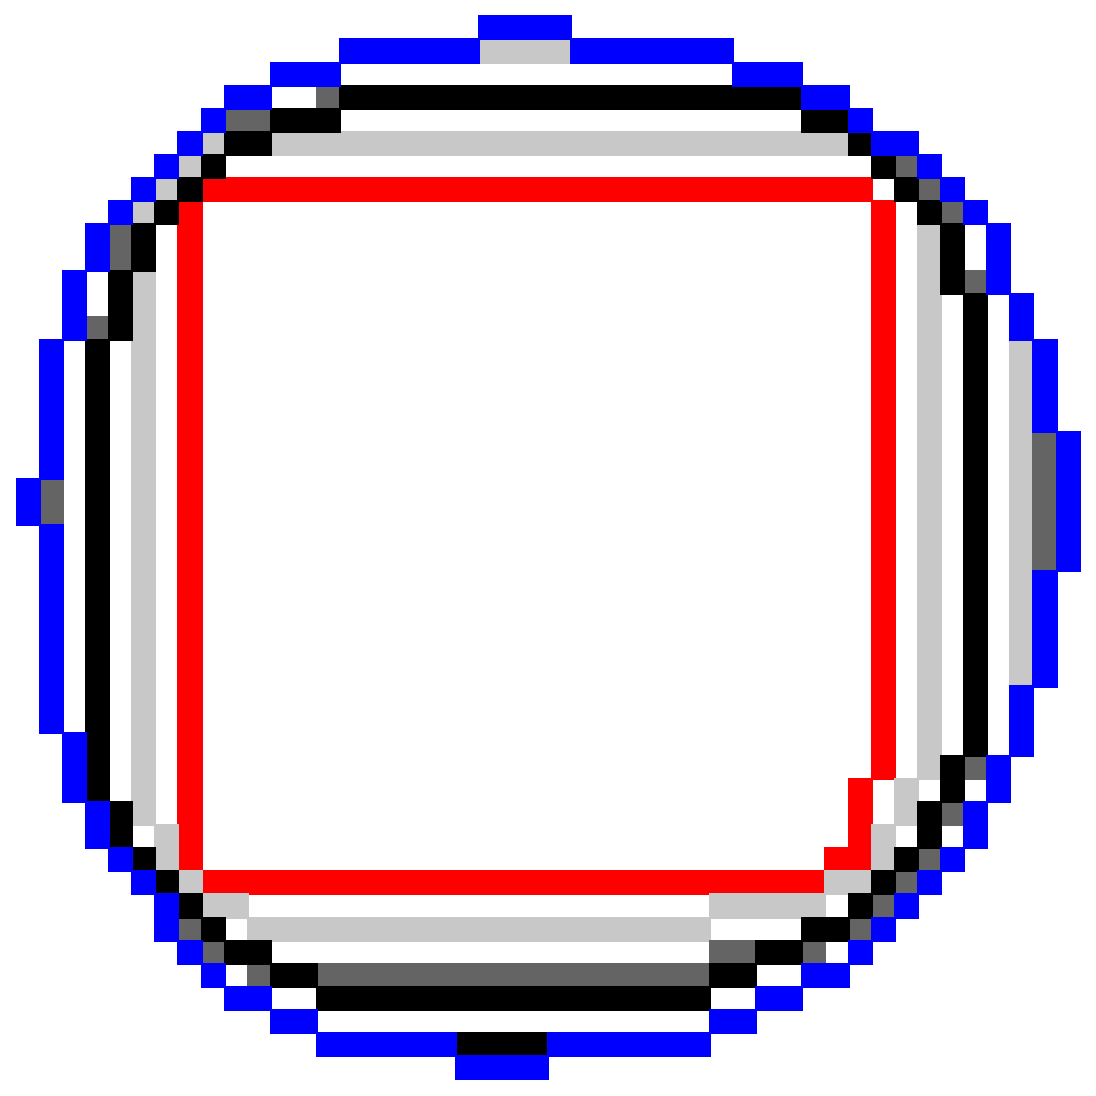
\includegraphics[scale=0.125]{images/local_search/square/h1.0/summary_flow.eps}
	}%
	\hspace{10pt}
	\subfloat[\label{}]{%
	\textbf{Missing figure}
	%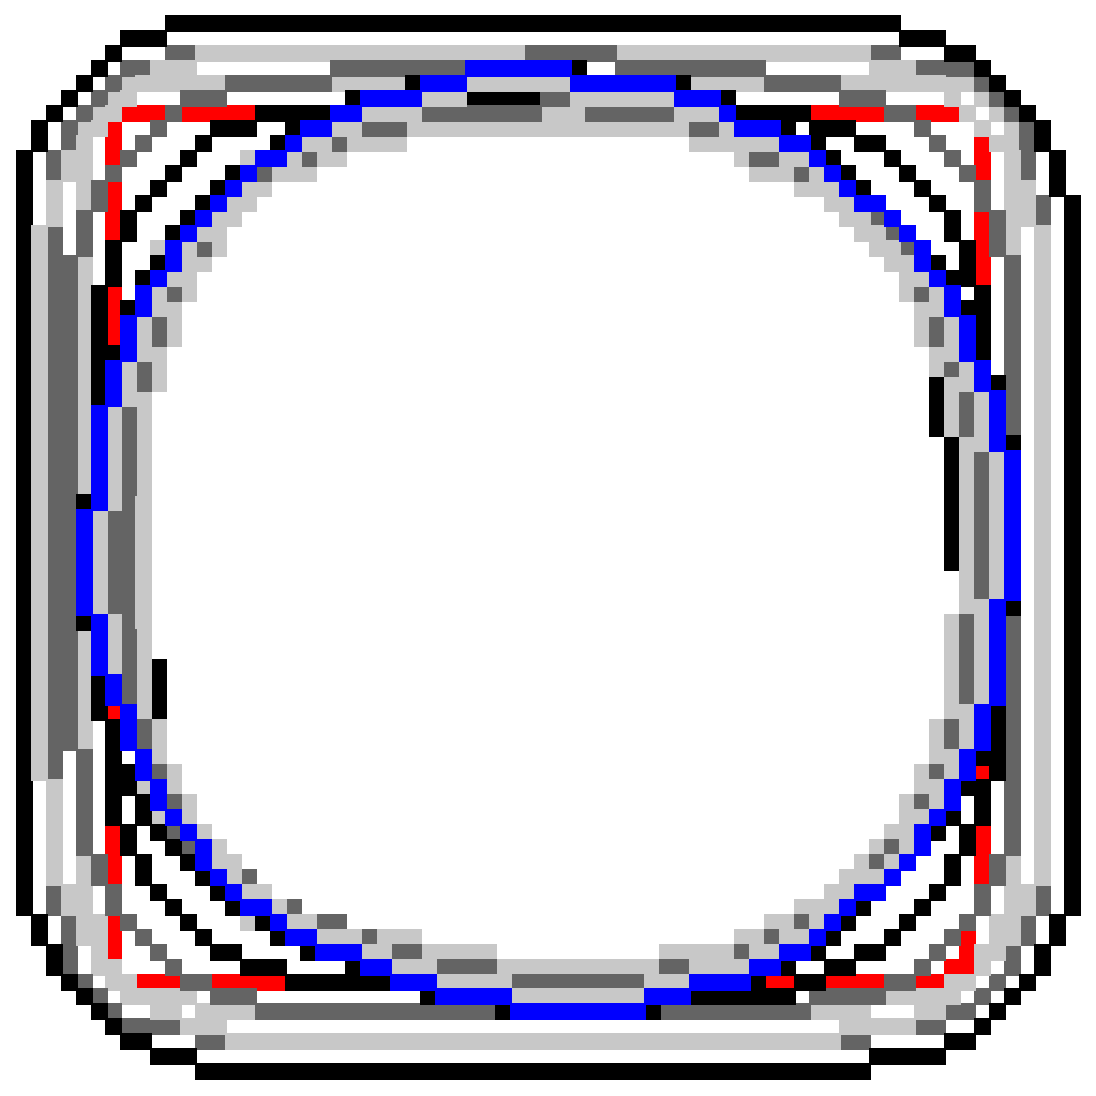
\includegraphics[scale=0.125]{images/local_search/square/h0.5/summary_flow.eps}
	}%
		\caption{Local combinatorial optimization process results for the square and flower shapes. Grid step $1.0$ in (a),(c) and $0.5$ in (b),(d).}	
		\label{fig:local-comb-square-results}
\end{figure}


The running time of algorithm \ref{alg:local-search} is summarized in
table \ref{tab:summary-local-comb-rtime}. All the experiments in this paper were executed in a five core $3.4Ghz$ cpu and the number of pixels in the triangle, square and flower shapes are respectively $841,1867,521$ for grid step $h=1.0$. Although its use in practical applications is limited, we
demonstrate that digital estimators are effective in its measurements
and the evolved flows behave as expected. We observe that is a
complete digital approach, and we do not suffer from discretization
and rounding problems, a common issue in continuous models.
Furthermore we have checked that this approach works
  indifferently with Integral Invariant curvature estimator and
  Maximal Digital Circular Arc curvature estimator. So the convergence
  of the digital curvature estimator seems to be the cornerstone to
  get a digital curve behaving like a continuous elastica.  In the
next section, we explore a more efficient approach.



\begin{figure}
\begin{minipage}[b]{0.5\textwidth}
\center
%\includegraphics[scale=0.35]{images/local_search/square/graph.eps}
	\textbf{Missing figure}
\caption{Elastica computation along iterations of algorithm \ref{alg:local-search}}
\label{fig:plot-elastica-local-search}
\end{minipage}\hspace{40pt}%
\begin{minipage}[b]{0.45\textwidth}
\center
\captionsetup{type=table}
\begin{tabular}{|l|c|c|}
\hline
& $h=1.0$ & $h=0.5$\\
\hline
Square & 747s (36s/it) & 7497s (202s/it)\\
\hline
Flower & 6946s (87s/it)  & 66376s (593s/it)\\
\hline
\end{tabular}
\caption{Running times for the local combinatorial optimization algorithm with $k=1,N=20$.}
\label{tab:summary-local-comb-rtime}
\end{minipage}
\end{figure}

\section{Digital Curvature Flow}

	Let $\Omega_C$ be the collection of connected digital sets in $\Omega$. Given a digital shape $S$, we wish to evolve it into a shape $S^\star$ similar to $S$ but with lower digital elastica energy. We recall the digital curvature estimator definition
	
\begin{align}
	\hat{\kappa}^2(y) &= c_1\Big( c_2 - | B_r(y) \cap S | \Big)^2, 
	\label{eq:curvature-estimator-pixels}
\end{align}

where $c_1=3/r^6$ and $c_2=\pi r^2/2$. Let $X,Y$ be the set of pixels and linels, respectively, in $\Omega$. We define the following binary model
		
\begin{align}
\text{Minimize}_{x,y} & \sum_{y}{c_1y \Big(c_2 - \sum_{x_j \in B_r(y)}{x_j}\Big)^2	 } + F(S,X_{=1} \cup Y_{=1}) \nonumber \\
\text{subject to} & \nonumber \\
& (X_{=1} \cup Y_{=1}) \in \Omega_C, \; x,y \in \{0,1\}^\Omega
\label{eq:general-binary-formulation}
\end{align}


where $F$ is some measure of similarity, e.g. distance, between initial shape $S$ and candidate solution. Such term is needed, otherwise the uninteresting empty set would be the optimal solution.

Formulation \eqref{eq:general-binary-formulation} is of order four, binary and non-convex. These properties make it a hard optimization problem. We are going to explore an alternative energy, which is a simplification of the former.

\subsection{A first model}

We note that the elastica can be decreased by attenuating non-flat regions. The idea is to evolve a flow $S^{(i)}$ where $S^{(i+1)}$ is derived from the minimization of the sum of the squared curvature at $S^{(i)}$. We exchange solving a fourth order energy to solve multiple second order problems. We still have to guarantee that solutions are connected. We handle this issue by limiting the optimization region to a subset of $\Omega$, namely the inner pixel boundary of  $S^{(i)}$.

\begin{definition}[Inner pixel boundary]
{
Given a digital shape $S$ embedded in a domain $\Omega$, we define its inner pixel boundary set $O(S)$ as
\begin{align*}
	O(S) = \left\{ \: x \; | \; x \in S, |\mathcal{N}_4(x) \cap S|<4 \: \right\},
\end{align*}
where $\mathcal{N}_4(x)$ denotes the $4$-adjacent neighbor set of $x$ (without $x$).
}
\end{definition}

In other words, each flow iteration decides which pixels in the inner boundary are to be removed and which are to be kept. To simplify notation, we denote the optimization region of $S^{(i)}$ as $O^{(i)}$. We define the foreground set $F^{(i)} = S^{(i)} \setminus O^{(i)}$.

In order to be symmetric, the curvature at some linel $y$ is computed on $R_m(S)$. We define $O_{r}^{(i)}(y) = O^{(i)} \cap B_r(y)$ and an analogous definition holds for $F_{r}^{(i)}(y)$. Expanding \eqref{eq:curvature-estimator-pixels}, we get 

	\begin{align*}
		\hat{\kappa}^2(y) &= c_1\Big( c_2 - \sum_{x_j \in B_r(y)} \big( {x_j} + |F_{r}^{(i)}(y)| \big) \Big)^2 \\
		\hat{\kappa}_{r}^2(y) &= c_1 \cdot \Big( C + 2\left( |F_{r}^{(i)}(y)| - c_2 \right) \sum_{x_j \in O_{r}^{(i)}(y)}{x_j} + \sum_{x_j \in O_{r}^{(i)}(y)}{x_j^2} + \sum_{ \substack{x_j,x_k \in O_{r}^{(i)}(p) \\ j<k} }{2x_jx_k}  \Big),
	\end{align*}
	
	where $C=c_2^2 - 2c_2 \cdot |F_{r}^{(i)}(y)| + |F_{r}^{(i)}(y)|^2$. We proceed by minimizing the sum of squared curvatures along $R_m(S)$. By ignoring constants and multiplication factors and using the binary character of the variables, we define the following family of energies
	
	\begin{align}
		E_m(X,S) = \sum_{y \in R_m(S)}{ \Big( { (1/2+ |F_{r}^{(i)}(y)|-c_2) \cdot \sum_{x_j \in O_{r}^{(i)}(y)}{x_j} } + \sum_{ \substack{x_j,x_k \in O_{r}^{(i)}(y) \\ j<k} }{x_jx_k} \Big) }.
		\label{eq:energy-family}
	\end{align}
	
	Each choice of $m$ generates a different flow, which is generaly described in the DCE algorithm \ref{alg:evolution-model}.



\begin{algorithm}[H]
 \SetKwData{It}{i}
 \SetKwData{MIt}{maxIt}
 \SetKwData{Delta}{delta}
 \SetKwInOut{Input}{input}\SetKwInOut{Output}{output}
 \SetKwComment{comment}{//}{}
 
 \Input{A digital set $S$; The ring number $m$; the maximum number of iterations \MIt;}
 \BlankLine
 $S^{(i)} \longleftarrow S$\;
 \While{ \It $<$ \MIt  }{ 	
	\comment{Expansion mode}
	\If{ \It is odd }{	 
	 	$Z^{(i)} \longleftarrow \argmin_Z E_m(Z,\overline{S^{(i)}})$\;
 		$S^{(i)} \longleftarrow F^{(i)} + \overline{Z^{(i)}}$\;
 		$S^{(i)} \longleftarrow \overline{S^{(i)}}$\;	 	
 	}
	\comment{Shrinking mode} 	
 	\Else{	
	 	$Z^{(i)} \longleftarrow \argmin_Z E_m(Z,S^{(i)})$\; 	
 		$S^{(i)} \longleftarrow F^{(i)} + \overline{Z^{(i)}}$\;
 	}
 	
	\It $\longleftarrow$ \It $+1$\;
	
 }
 \label{alg:evolution-model} 
 \caption{Digital curvature evolution algorithm (DCE).}
\end{algorithm}



Recall that II estimates curvature by computing the difference between half of the estimation ball area and the intersection of such ball with the shape.  In particular, regions of positive curvature have fewer pixels in its intersection set than on its complement wrt the estimation ball. This implies that variables in such regions are labeled one, as the unbalance grows otherwise. We attenuate curvature if we shift the center of the estimation ball towards the interior of the shape, which means removing the labeled one pixels. That's why we take the complement of the optimization solution. 

The same reasoning applies for non-convex parts. Indeed, concave regions are convex in the shape complement. In the expasion mode we apply the same reasoning on the image complement, and by doing this we are able to handle concavities. It is called expansion mode because the optimization region, in this case, is the outer pixel boundary of the original shape. 


\begin{table}
  \center
  \begin{tabular}{|c|c|c|c|} \hline
    shrink mode &    $\kappa \gg 0$ & $\kappa \geq 0$ &  $\kappa < 0$ \\ \hline
    $Z$ & $x_k=1$ & $x_k \in \{0,1\}$ & $x_k=0$ \\ \hline
    $S^{(i+1)} \leftarrow S^{(i)} \setminus Z$ & eroded & prob. eroded & unchanged  \\ \hline \hline
    expansion mode &    $\bar{\kappa} \gg 0$ & $\bar{\kappa} \geq 0$ & $\bar{\kappa} < 0$ \\ \hline
    $\bar{Z}$ & $\bar{x}_k=1$ & $\bar{x}_k \in \{0,1\}$ & $\bar{x}_k=0$ \\ \hline
    $S^{(i+1)} \leftarrow \overline{\bar{S}^{(i)} \setminus \bar{Z}}$ & dilated & prob. dilated & unchanged \\ \hline 
  \end{tabular}
  
  \label{tab:flow-summary}	  
  \caption{  Since the curvature is negated when reversing the curve (i.e. $\bar{\kappa}=-\kappa$), this process can only shrink  convex parts in shrink mode and expand concave parts in expansion mode.}

\end{table}


In figure \ref{fig:m1-square-flow} we see some results for the DCE algorithm  with $m=1$. We observe a global movement towards roundness, but with several artifacts. We minimize the effects of a jaggy boundary by including a length penalization, weighted by some coefficient $\alpha$. Nonetheless, a higher estimation ball radius creates unstable shapes. In fact, the estimator is very sensitive in regions of low squared curvature, and its precisely in those regions which spurious pixels are included.


\begin{figure}[!ht]
\center
\begin{minipage}[b]{0.33\textwidth}
	\subfloat[$r=3, \alpha=0$\label{}]{%
	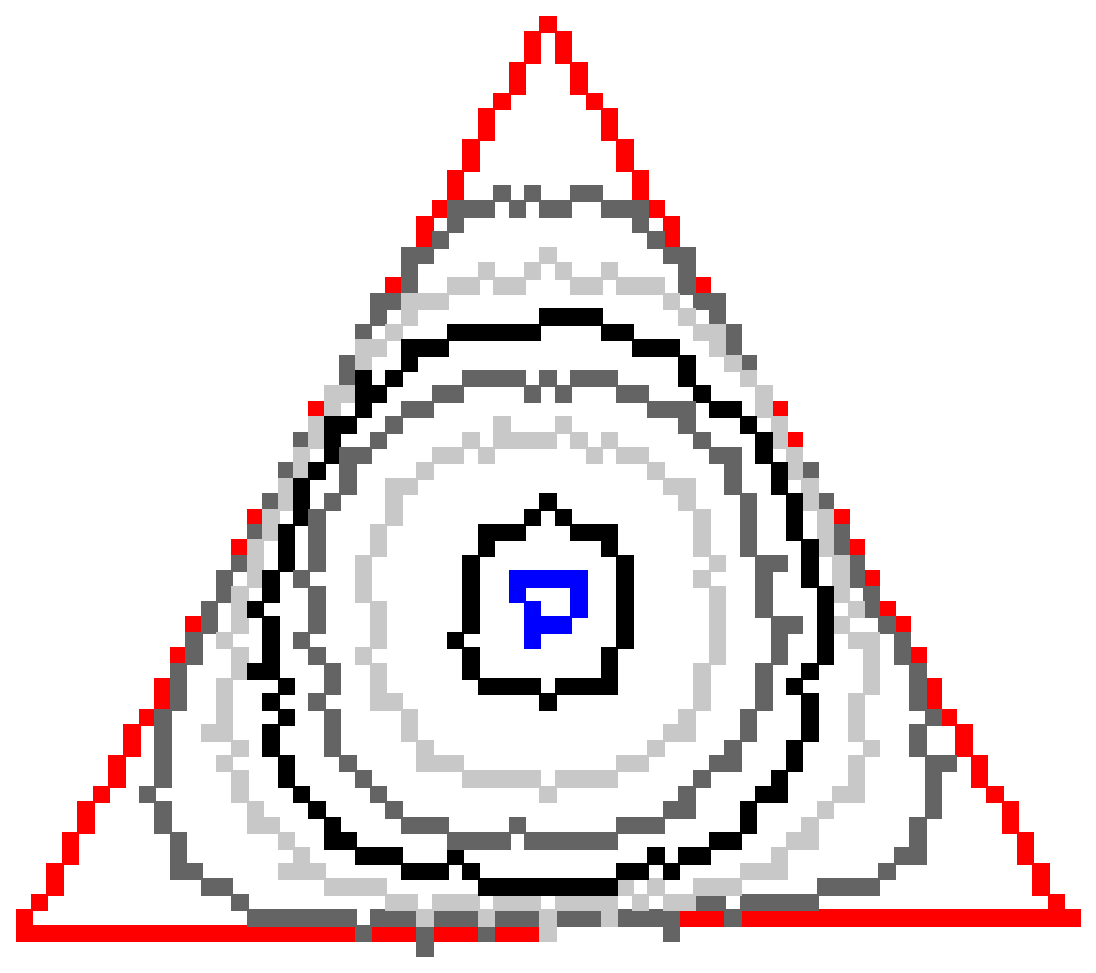
\includegraphics[scale=0.2]{images/flow/length-radius-effect/triangle-r3-nolength/summary_flow.eps}
	}%
\end{minipage}%
\begin{minipage}[b]{0.33\textwidth}
	\subfloat[$r=3, \alpha=0.15$\label{}]{%
	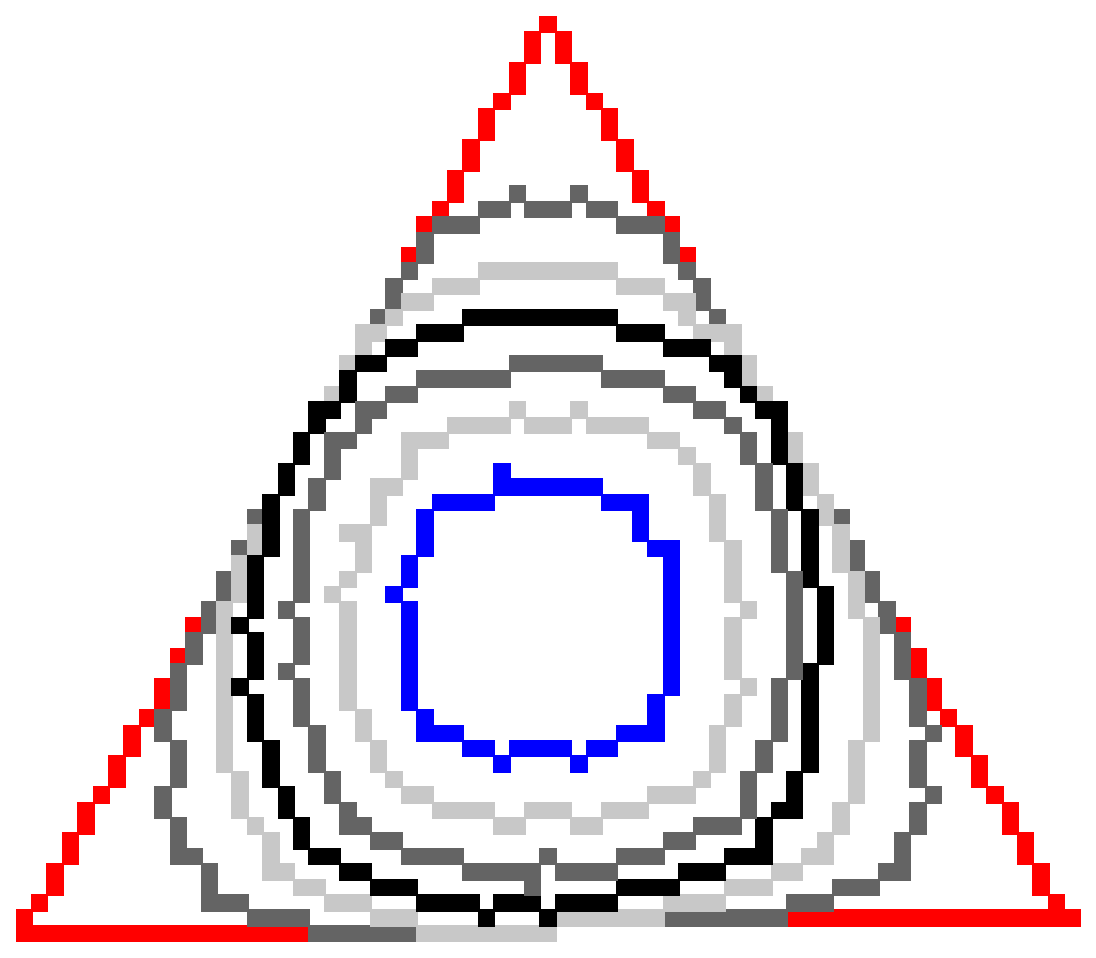
\includegraphics[scale=0.2]{images/flow/length-radius-effect/triangle-r3-length0.15/summary_flow.eps}
	}%
\end{minipage}%
\begin{minipage}[b]{0.33\textwidth}
	\subfloat[$r=5, \alpha=0.15$\label{}]{%
	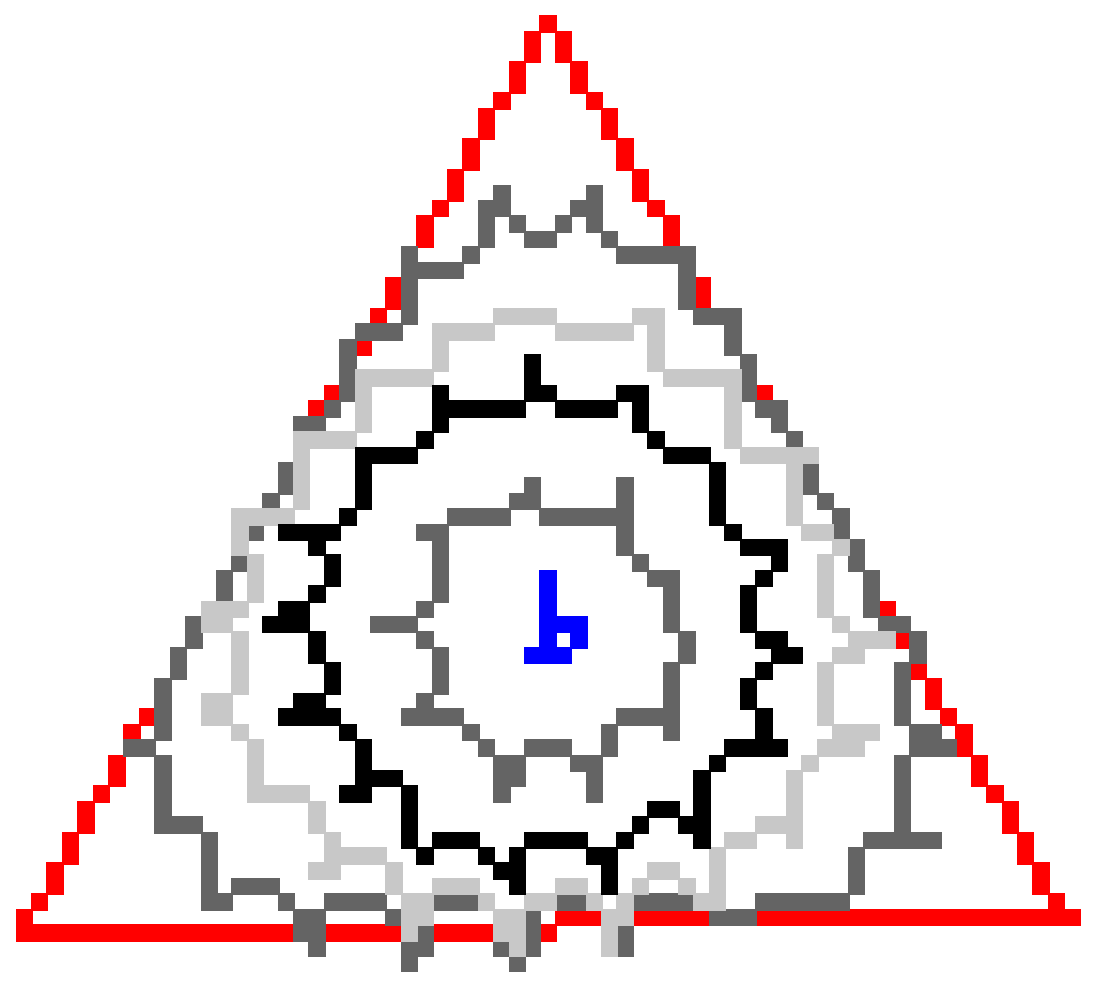
\includegraphics[scale=0.2]{images/flow/length-radius-effect/triangle-r5/summary_flow.eps}
	}%
\end{minipage}%
\caption{The algorithm is very sensitive to the variations of the estimator, which are particularly important in regions of low squared curvature. Artifacts are reduced with a length penalization but increases if we use a higher ball radius. }
\label{fig:m1-square-flow}
\end{figure}


\subsection{A more stable model}

In the previous section we notice that the algorithm produces shapes with many artifacts due to the sensitiveness of the estimator on regions of low squared curvature. We argue that, evaluating the estimation ball along farther ring sets we skip those sensitive areas by focusing the optimization process only on those regions of highest squared curvature value. 

\jaco{Motivation in digital geometry of why it makes sense to compute things farther.}



\begin{figure}[!ht]
\center
\center
\begin{minipage}[b]{0.33\textwidth}
	\subfloat[$r=5, m=1$\label{}]{%
	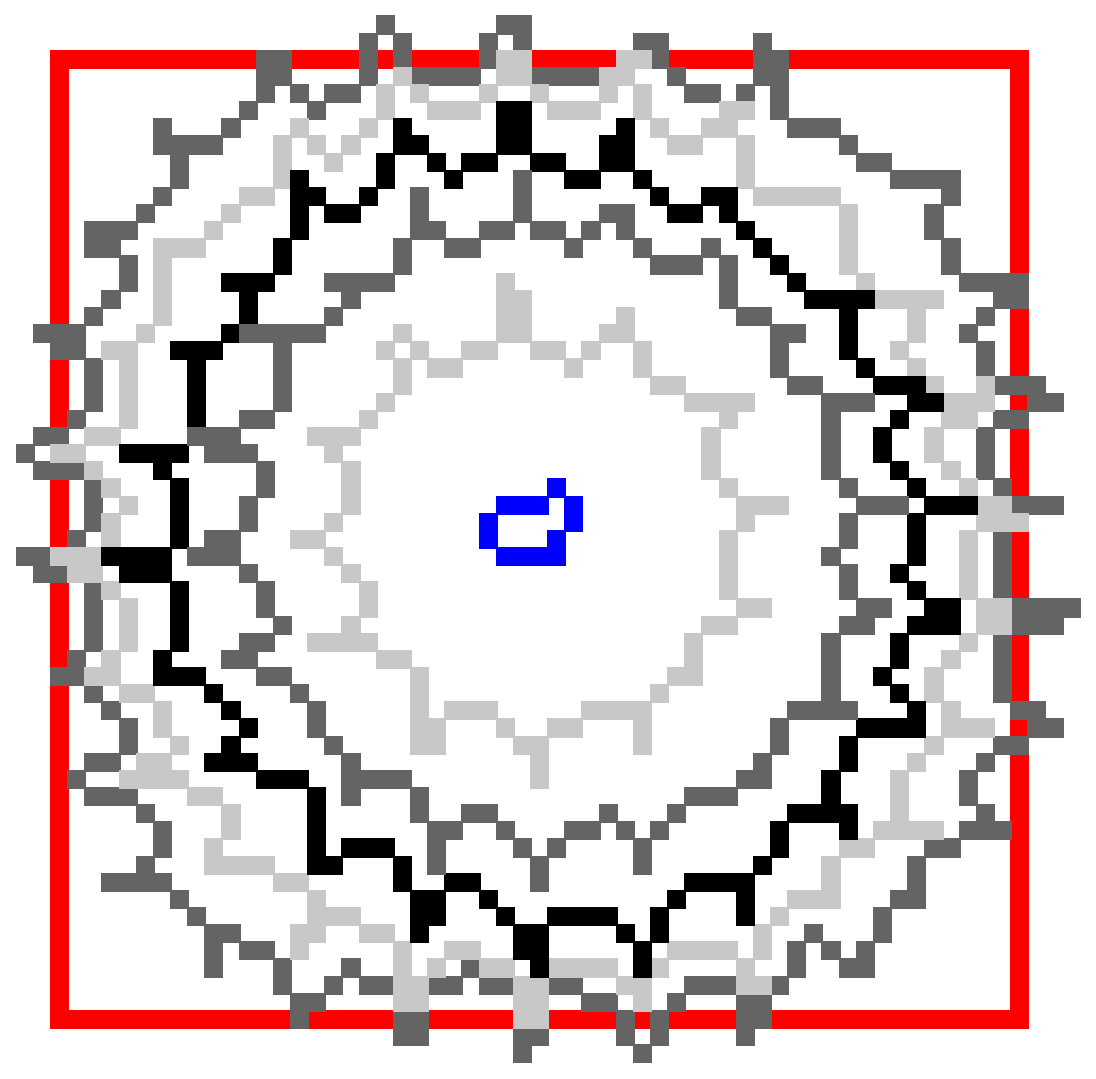
\includegraphics[scale=0.2]{images/flow/farther-rings/square-r5-l1/summary_flow.eps}
	}%
\end{minipage}%
\begin{minipage}[b]{0.33\textwidth}
	\subfloat[$r=5, m=2$\label{}]{%
	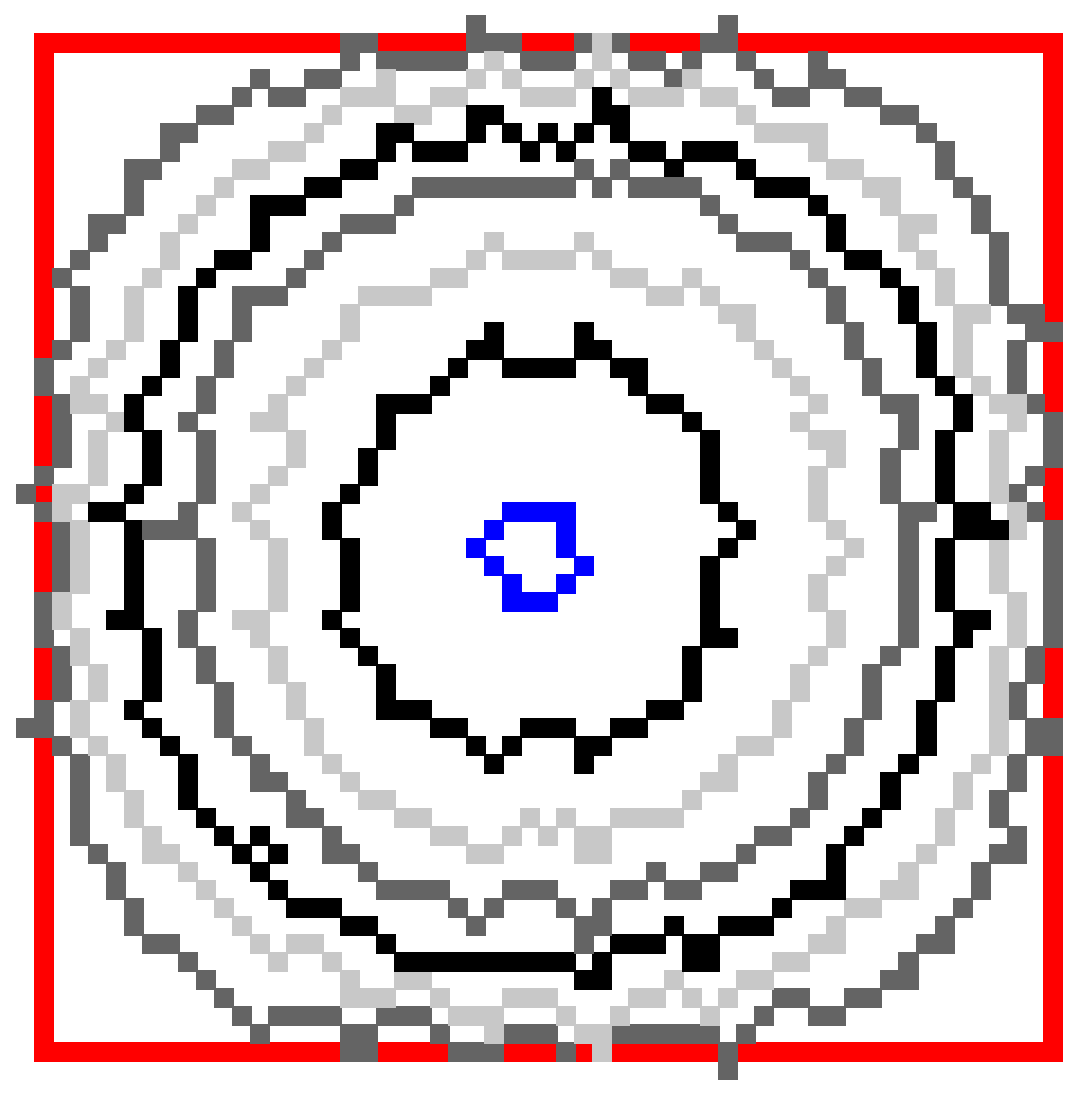
\includegraphics[scale=0.2]{images/flow/farther-rings/square-r5-l2/summary_flow.eps}
	}%
\end{minipage}%
\begin{minipage}[b]{0.33\textwidth}
	\subfloat[$r=5, m=3$\label{}]{%
	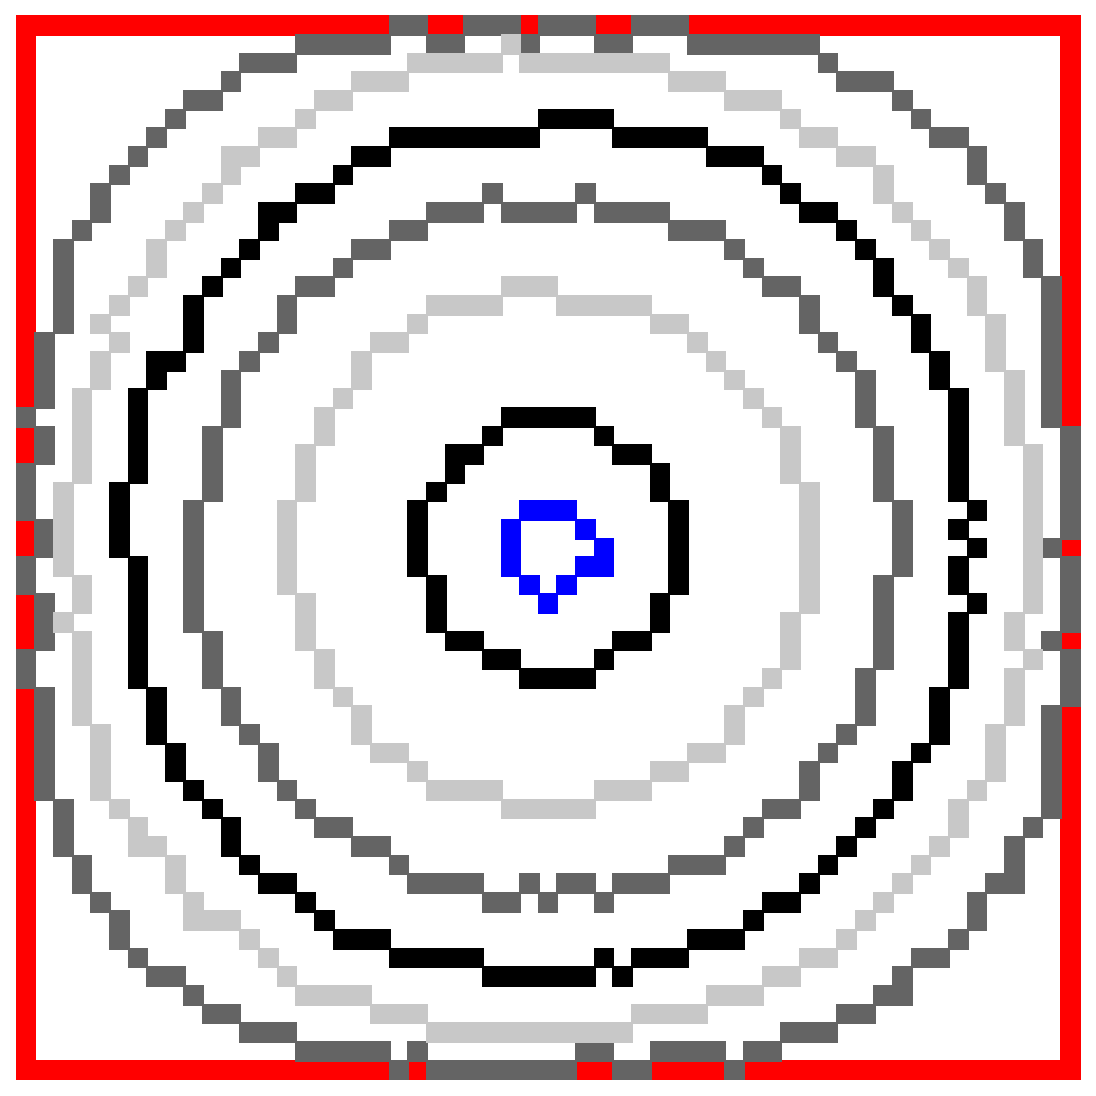
\includegraphics[scale=0.2]{images/flow/farther-rings/square-r5-l3/summary_flow.eps}
	}%
\end{minipage}%
\label{fig:mx-square-flow}
\caption{By positioning the estimation ball on farther rings, we minimize artifacts creation. }
\end{figure}

In our experiments, the best results are obtained by executing DCE algorithm with $m=r$, where $r$ is the estimation ball radius. In plot \ref{fig:mx-elastica-plots}, we observe how the elastica evolves along the iterations. If the radius is too large, the elastica increases starting from a critical point $p$. That's what happens for the triangle, in which the flow converges to a single point. 


\begin{figure}[!ht]
\center				
		\setcounter{subfigure}{-3}
		\subfloat[$r=3,h=0.5$]{%
		\subfloat{%
		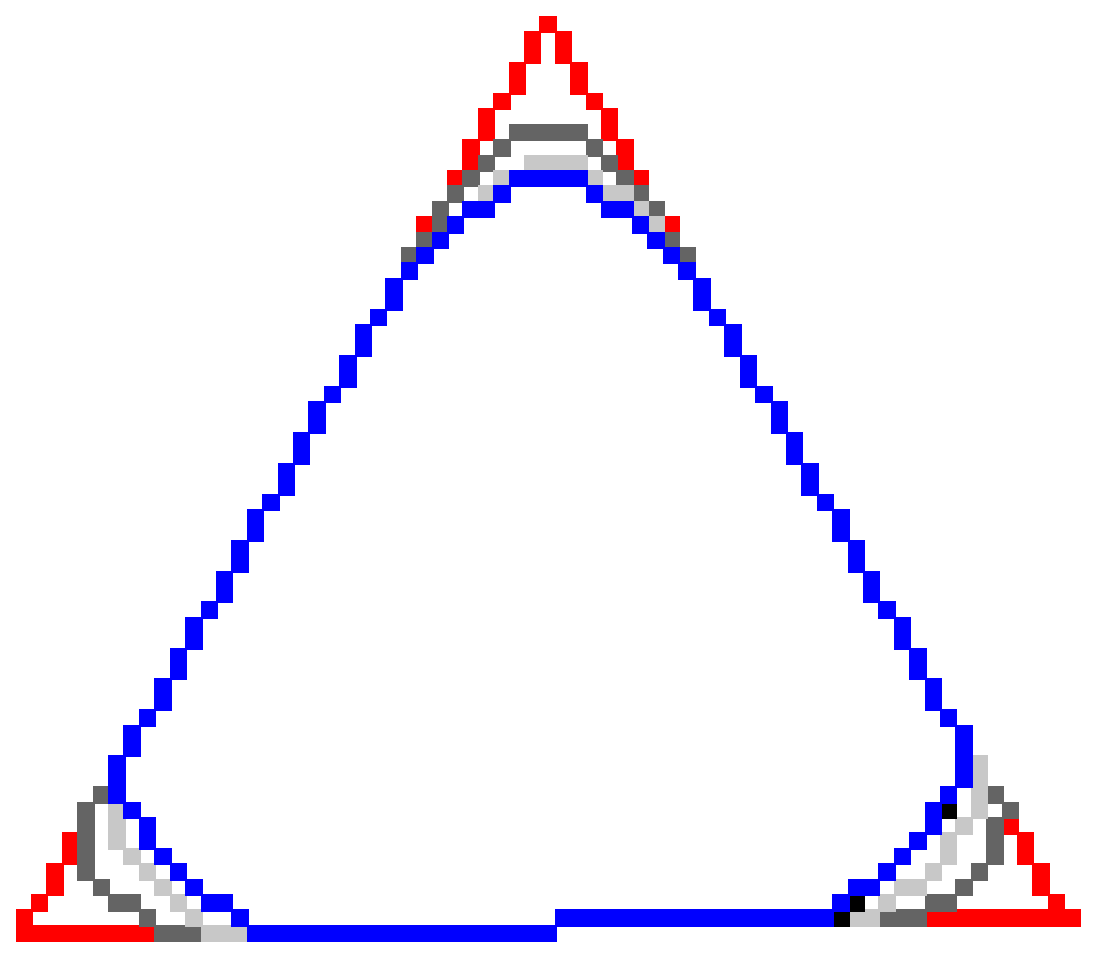
\includegraphics[scale=0.2]{images/flow/grid-radius-effect/triangle/r3-h0.5/summary_flow.eps}
		}%
		\hspace{15pt}
		\subfloat{%
		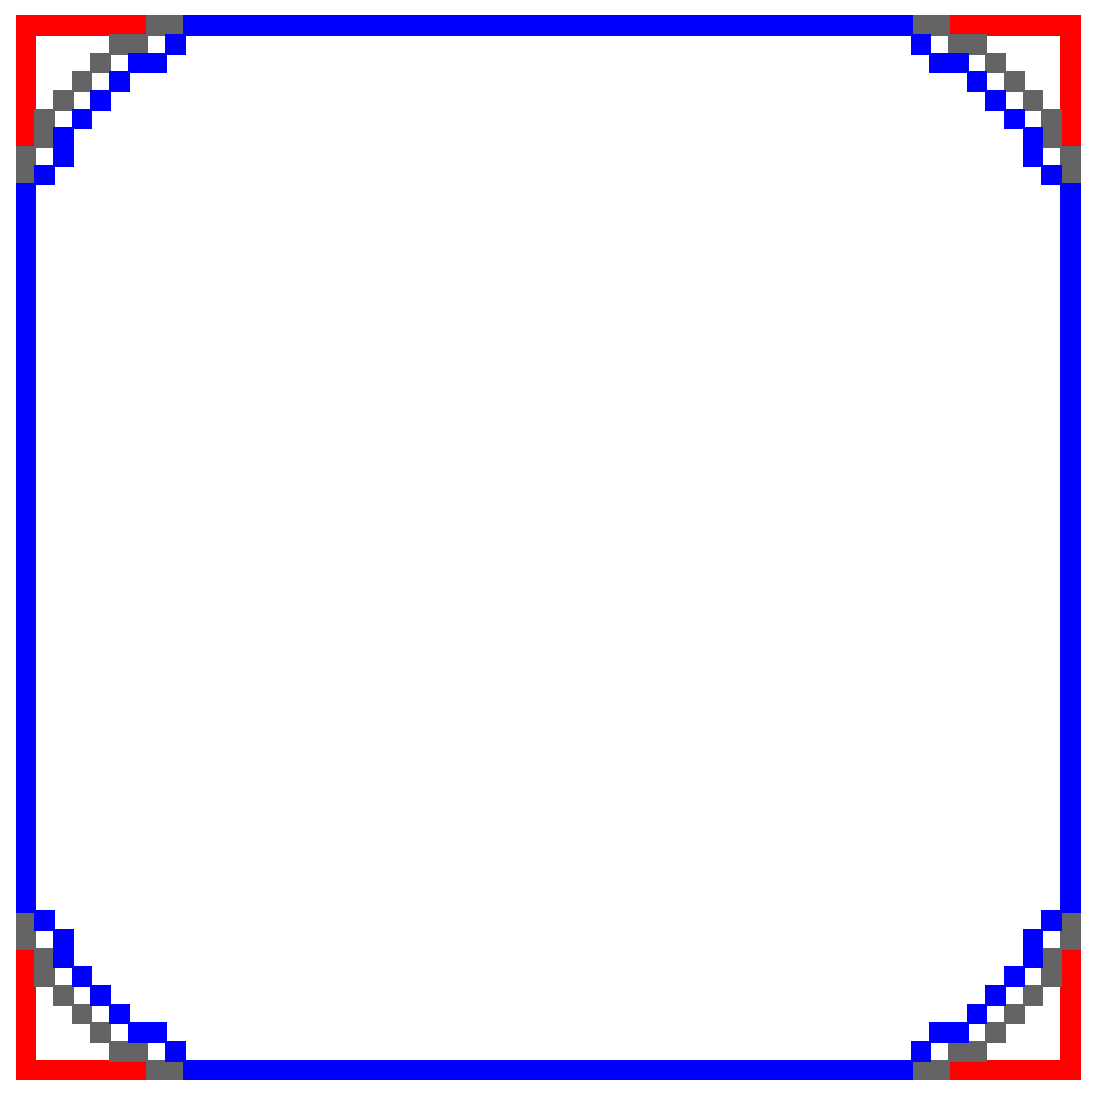
\includegraphics[scale=0.15]{images/flow/grid-radius-effect/square/r3-h0.5/summary_flow.eps}}%
		\hspace{15pt}
		\subfloat{%
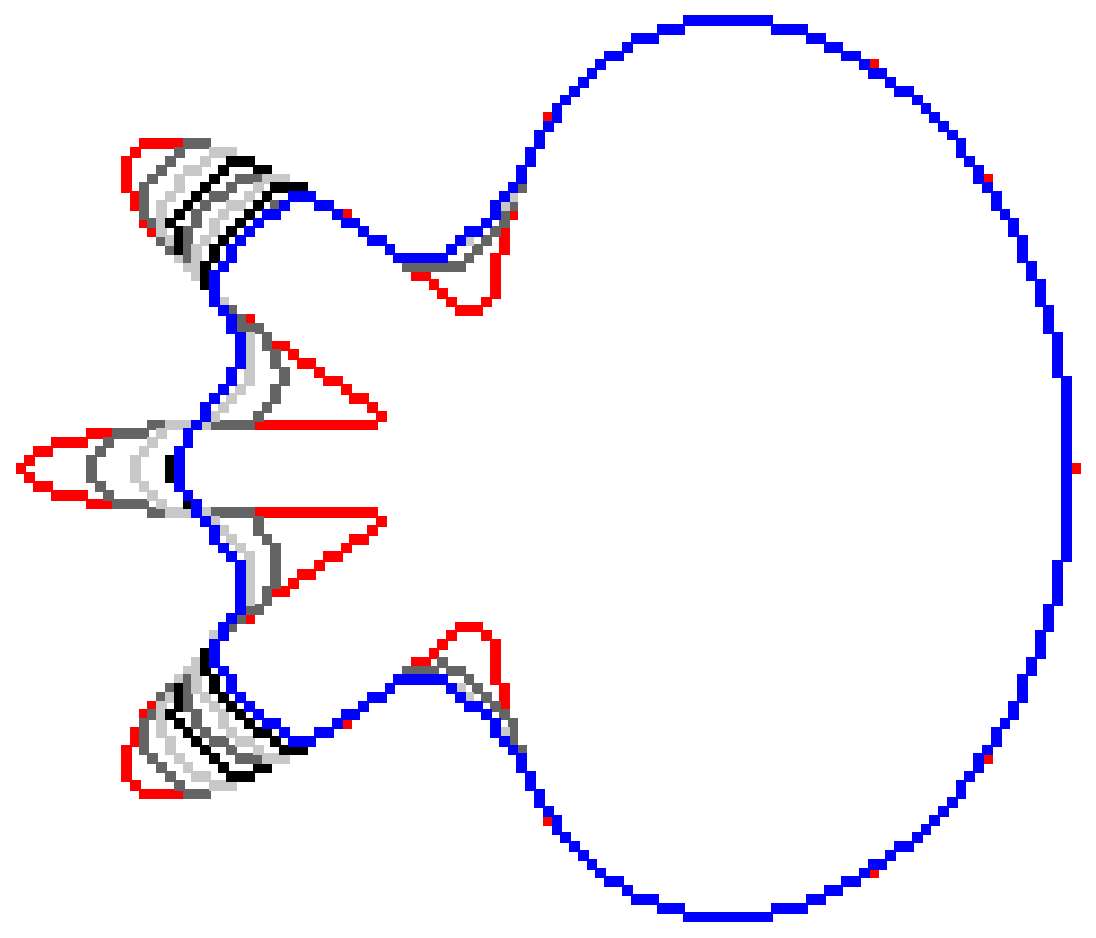
\includegraphics[scale=0.2]{images/flow/grid-radius-effect/flower/r3-h0.5/summary_flow.eps}}%
		}		
	
		\setcounter{subfigure}{-2}
		\subfloat[$r=5,h=0.5$]{%
		\subfloat{%
		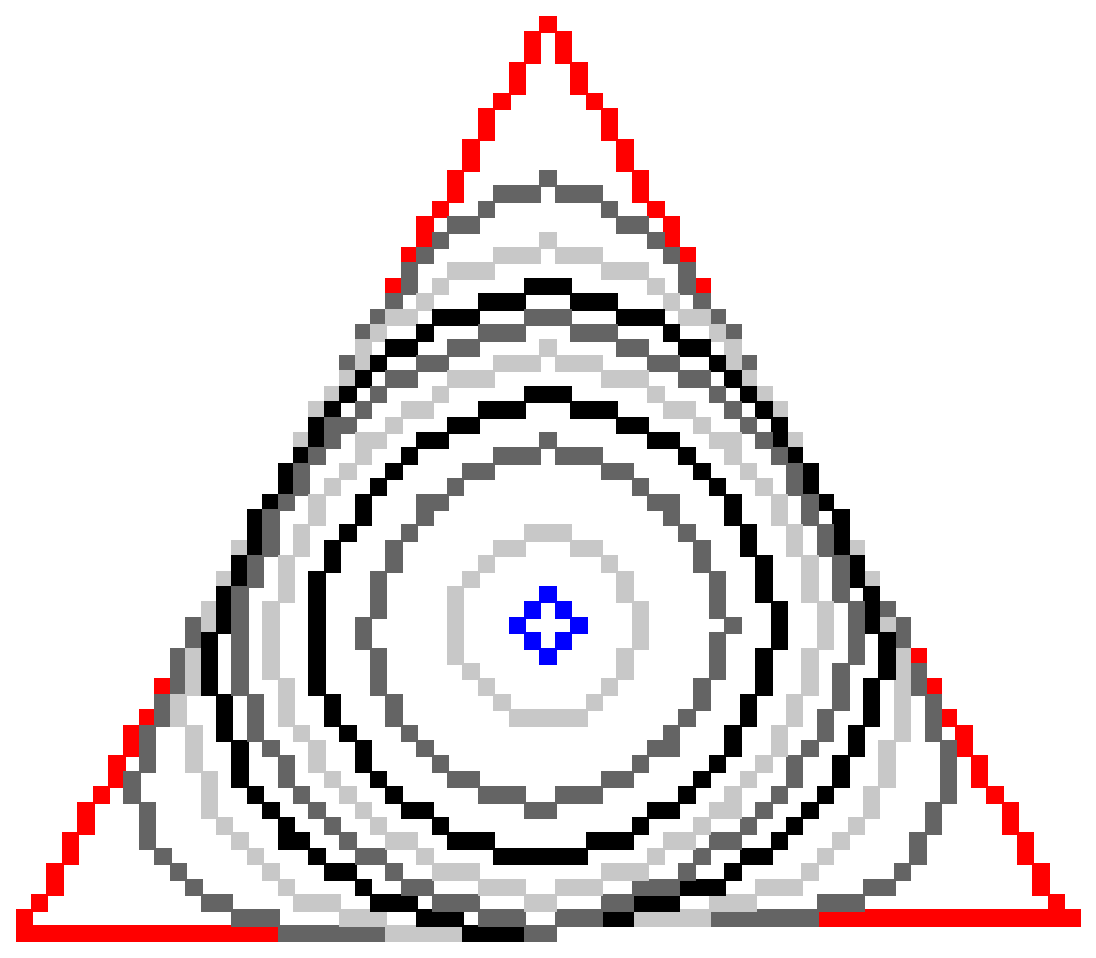
\includegraphics[scale=0.2]{images/flow/grid-radius-effect/triangle/r5-h0.5/summary_flow.eps}
		}%1
		\hspace{15pt}
		\subfloat{%
		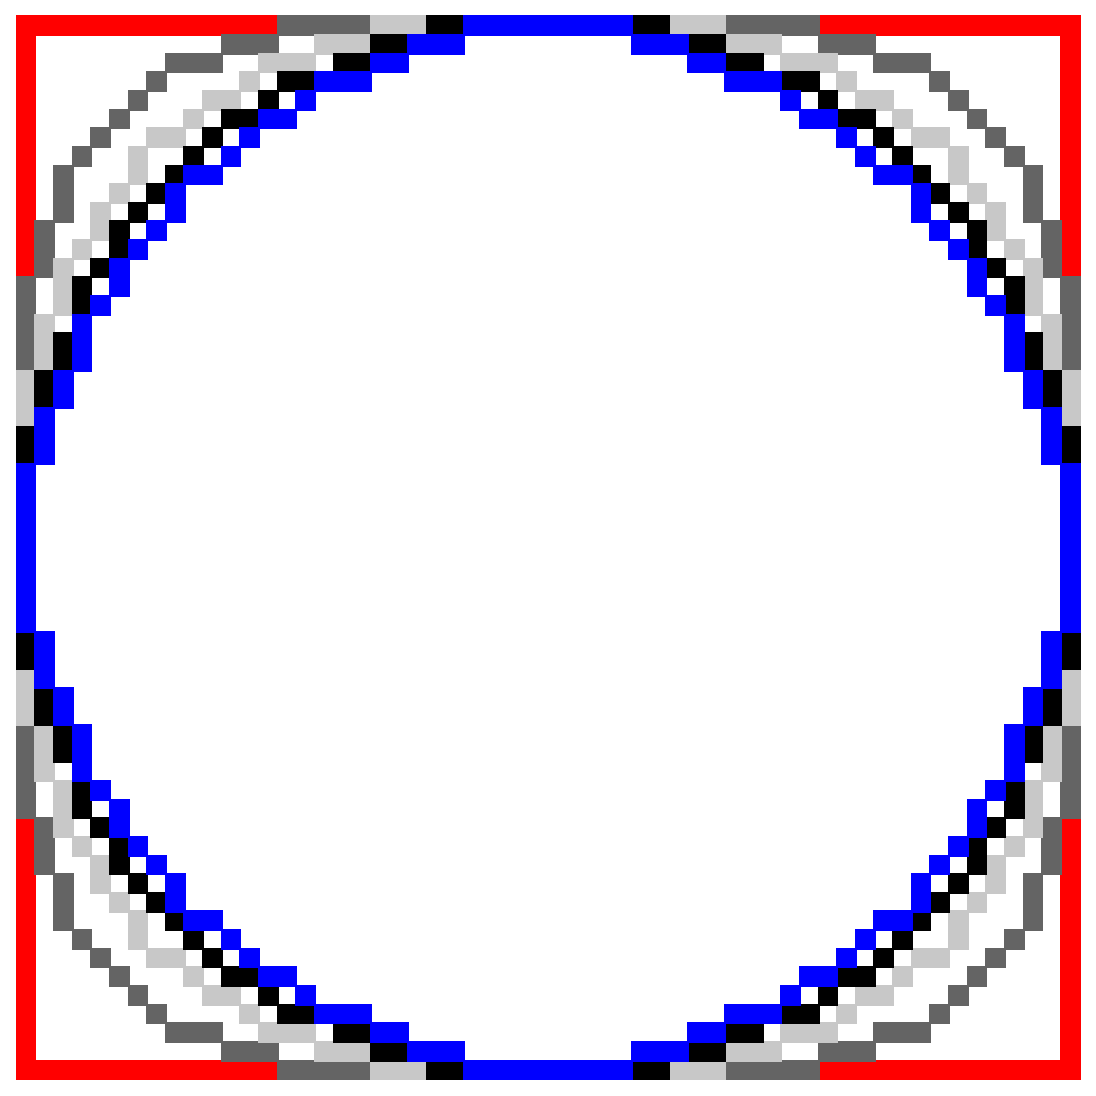
\includegraphics[scale=0.15]{images/flow/grid-radius-effect/square/r5-h0.5/summary_flow.eps}}%
		\hspace{15pt}
		\subfloat{%
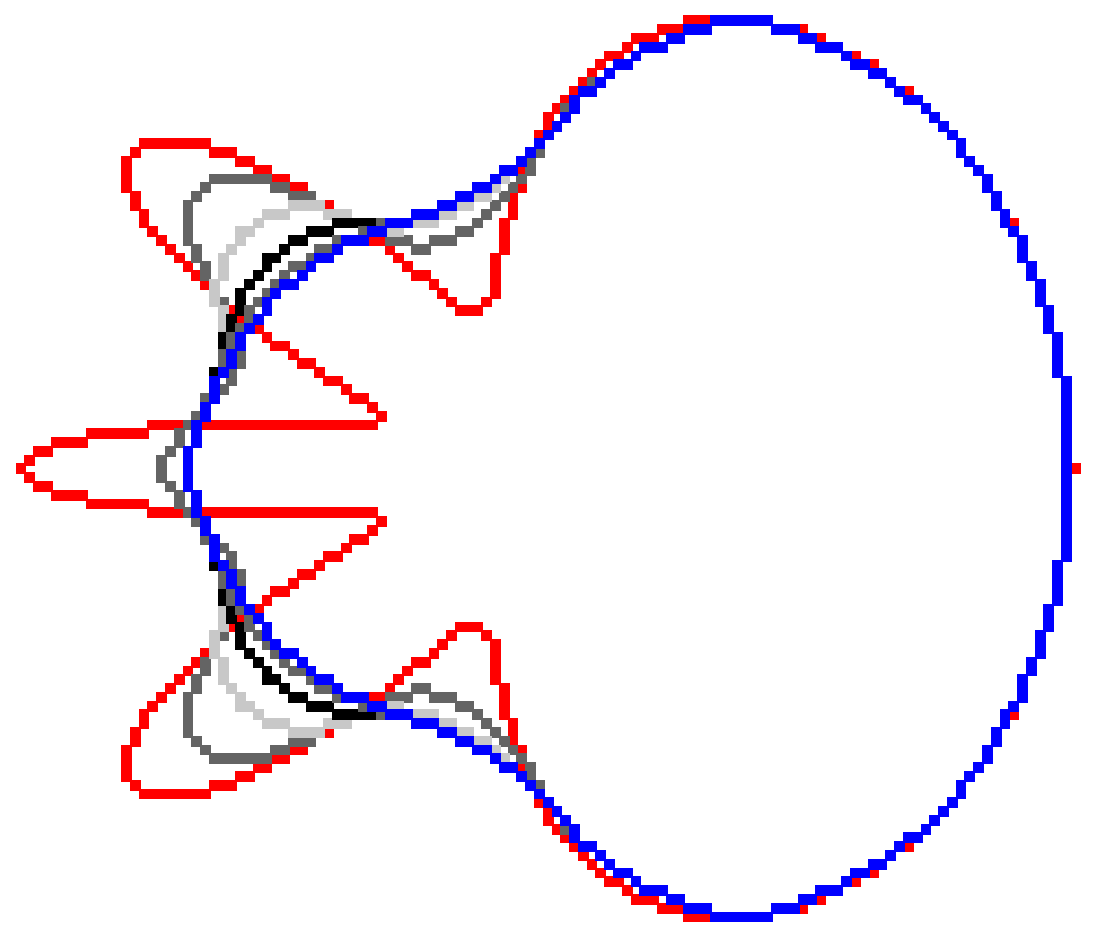
\includegraphics[scale=0.2]{images/flow/grid-radius-effect/flower/r5-h0.5/summary_flow.eps}}%
		}				
		
		
\label{fig:mx-flow-gs-radius-effect}
\caption{The choice of radius has an impact on the flow. In the figures, the flow ceases to evolve for all shapes  when $r=3$ (a). In figure (b), for $r=5$, the triangle evolves to a single point, while the other shapes stop  evolution, but further than in (a). }
\end{figure}

\begin{figure}[!ht]
\center
\includegraphics[scale=0.5]{images/flow/elastica-energy-plot/r5h05.eps}
\caption{Elastica computation along the iterations for different shapes. If radius is too large, elastica may increase after a certain number of iterations. }
\label{fig:mx-elastica-plots}
\end{figure}

\begin{figure}[!ht]
\center
\subfloat[]{%
	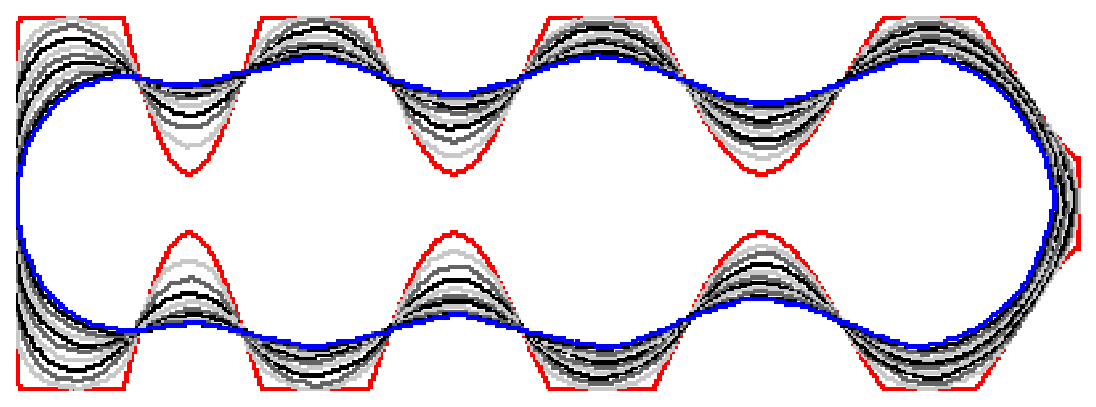
\includegraphics[scale=0.5]{images/flow/faster-high-curvature/summary_flow.eps}}\\%
\subfloat[]{%
		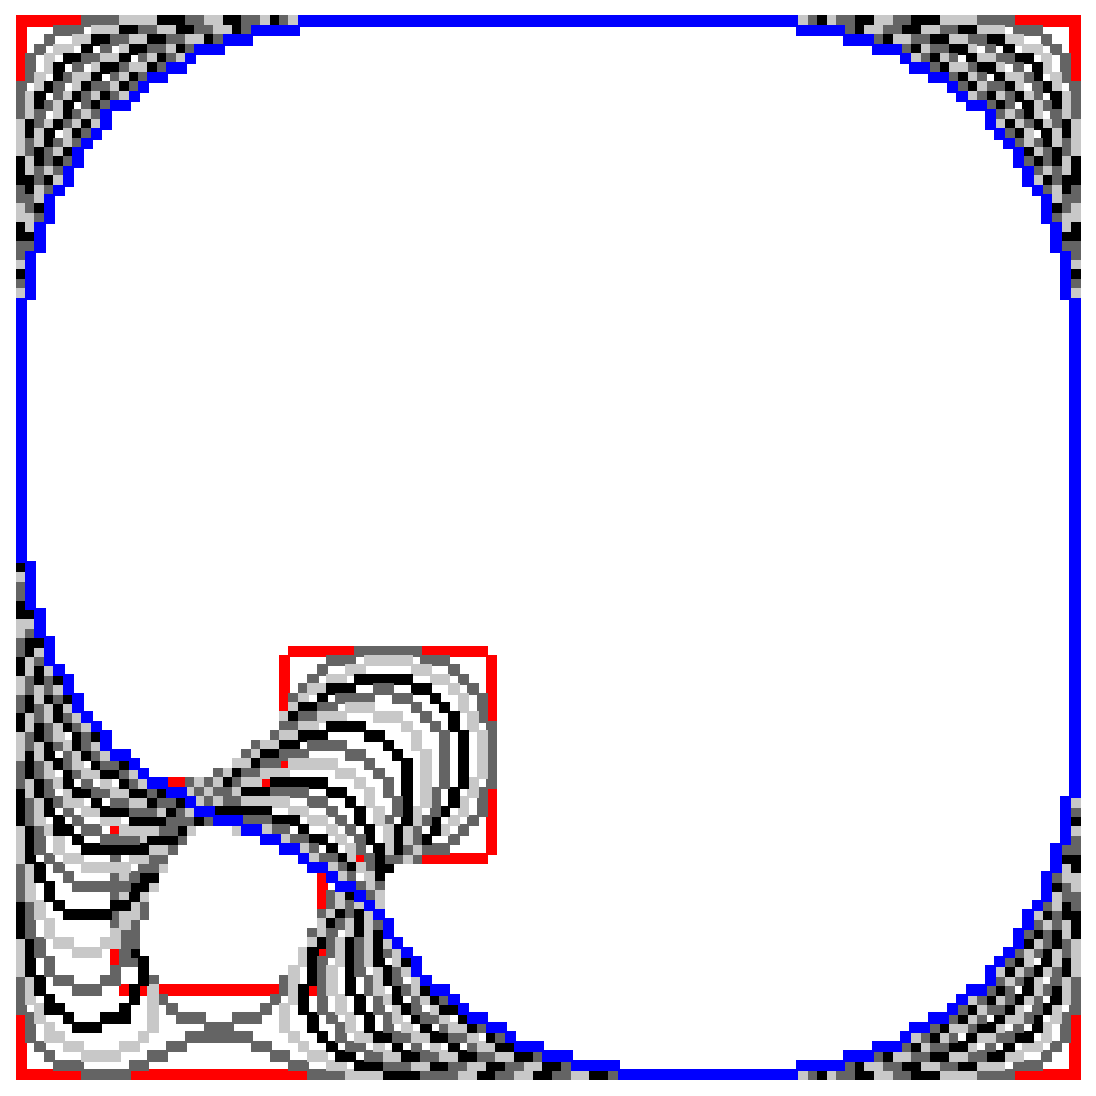
\includegraphics[scale=0.25]{images/flow/fill-holes/summary_flow.eps}}%%1
\label{fig:mx-speed-variation-hole-filling}
\caption{High curvature regions evolves faster than lower ones (a). The flow can handle topological changes (b). }
\end{figure}


\subsection{Optimization method}

Let $f$ be a function of $n$ binary variables with unary and pairwise terms, i.e.

\begin{align*}
f(y_1,\cdots, y_n) = \sum_{j}{f_j(y_j)} + \sum_{j < k}{f_{j,k}(y_j,y_k)}
\end{align*}

Function $f$ is submodular if and only if the following inequality holds for each pairwise term $f_{j,k}$ \cite{kolmogorov04whatenergies}

\begin{align*}
	\quad f_{j,k}(0,0) + f_{j,k}(1,1) \leq f_{j,k}(0,1) + f_{j,k}(1,0)
\end{align*}

Energy $E_m$ is non-submodular and optimizing it is a difficult problem, which
constrained us to use heuristics and approximation algorithms. The QPBO method \cite{rother07qpbo} transforms the 
original problem in a max-flow/min-cut formulation and returns a full optimal labeling for submodular energies. For
non-submodular energies the method is guaranteed to return a partial labeling with the property that the set of labeled
variables is part of an optimal solution. That property is called partial optimality.

In practice, QPBO can leave many pixels unlabeled. There exist two extensions of QPBO that ameliorate this limitation: QPBOI
(improve) and QPBOP (probe). The first is an approximation method that is guaranteed to not increase the energy, but we
lost the property of partial optimality. The second is an exact method which is reported to label more variables than
QPBO. 

The percentage of unlabeled pixels by QPBOP for $E_1$ is quite high, but the percentage decreases to zero as we set $m$ equal to $r$. Therefore, we are more confident to take the solution for values of $m$ close to $r$. However, the manner which it varies across $m$ values differs from shape to shape, as it's illustrated in figure \ref{fig:unlabeled-versus-iterations}. 

We have used QPBOI to solve $E_m$. Naturally, in the case that all pixels are labeled by QPBOP, QPBOI returns the same labeling as QPBOP. 


\begin{figure}[!htp]
\center
\begin{minipage}[b]{0.5\textwidth}
\subfloat[]{ \includegraphics[scale=0.35]{images/optimization/unlabeled-iterations/radius-3/plot-model-square-concavities-probe.eps}}\\%
\subfloat[]{ \includegraphics[scale=0.35]{images/optimization/unlabeled-iterations/radius-5/plot-model-square-concavities-probe.eps}}\\%
\subfloat[]{ \includegraphics[scale=0.35]{images/optimization/unlabeled-iterations/radius-7/plot-model-square-concavities-probe.eps}}%
\end{minipage}%
\begin{minipage}[b]{0.5\textwidth}
\subfloat[]{ \includegraphics[scale=0.35]{images/optimization/unlabeled-iterations/radius-3/plot-model-flower-concavities-probe.eps}}\\%
\subfloat[]{ \includegraphics[scale=0.35]{images/optimization/unlabeled-iterations/radius-5/plot-model-flower-concavities-probe.eps}}\\%
\subfloat[]{ \includegraphics[scale=0.35]{images/optimization/unlabeled-iterations/radius-7/plot-model-flower-concavities-probe.eps}}%
\end{minipage}
\caption{The number of unlabeled pixels by QPBOP remains high for lower values of $m$, and goes to zero when $m=r$. We observe the same behaviour for different radius values.}
\label{fig:unlabeled-versus-iterations}
\end{figure}

\begin{figure}
\center
\includegraphics[scale=0.5]{images/optimization/pairwise-ratio/plot-pairwiseratio-lowerHigher-concavities-probe.eps}
\caption{We plot the ratio of pairwise terms among all $\binom{|X|}{2}$ combinations. The highest ring has rougly half the number of pairwise terms  than the lowest ring.}
\end{figure}



\section{Application in image segmentation}

We present an application in supervised image segmentation for the digital evolution described in the previous section. We include a data fidelity $g(\cdot)$ and a length penalization $s(\cdot)$ terms in energy $E_m$. At iteration $i$, we minimize

\begin{align}			
	\min_{Y^{(i)}} \sum_{y \in Y^{(i)}}{\Big( \gamma \cdot g(y) + \alpha \cdot s(y) \Big)} + \sum_{y \in R_r(S^{(i)})}{ \beta \cdot \hat{\kappa}_{r}^2(y)}.
	\label{eq:boundary-correction-energy}
\end{align}
	
	Let $\mathcal{N}_4(y)$ denote the four neighborhood of pixel $y$. Length penalization is defined as
	
	
	\begin{align*}
		s(y)=\sum_{y_j \in \mathcal{N}_4(y)}{ t(y_j) }, \quad \text{where } t(y_j) = \left\{\begin{array}{ll}
		(y-y_j)^2, & \text{if } y_j \in O_{r}^{(i)}\\
		(y-0), & \text{if } y_j \in F_{r}^{(i)}\\
		(y-1), & \text{otherwise }
		\end{array}\right.
	\end{align*}
	
	Given foreground and background seeds selected by the user, we derive mixed gaussian distributions  of color intensities $G_f$ and $G_b$, and we define the data fidelity term as
	
	\begin{align*}
		g(y) = -(1-y)\log{G_f(I(y))} - y\log{G_b(I(y))}
	\end{align*}
	
	Notice that data and length terms are defined in such a way in order to comply with DCE algorithm, in which we take the complement of the optimal solution. 
	
	
\begin{algorithm}[H]
 \SetKwData{It}{i}
 \SetKwData{MIt}{maxIt}
 \SetKwData{Tol}{tolerance}
 \SetKwData{Delta}{delta}
 \SetKwInOut{Input}{input}\SetKwInOut{Output}{output}
 \SetKwComment{comment}{//}{}
 
 \Input{An image $I$; seed mask $M$; The estimation ball radius $r$; data $(\gamma)$, length $(\alpha)$ and squared curvature $(\beta)$ weights; initial dilation $d$; stop condition value \Tol; the maximum number of iterations \MIt;}
 \BlankLine

 $S^{(i)} \longleftarrow$ GrabCut($I,M$)\;
 $S^{(i)} \longleftarrow $ dilate(I,d)\; 
 \While{ \It $<$ \MIt \bf{and} \Delta $>$ \Tol  }{ 	
 	$S^{(i+1)} \longleftarrow $ DCE($S^{(i)},\gamma,\alpha,\beta$)\;
 	\Delta $\longleftarrow |S^{(i)} - S^{(i+1)}|$\;

	\It $\longleftarrow$ \It $+1$\;
	
 }
 \label{alg:contour-correction} 
 \caption{Contour correction algorithm.}
\end{algorithm}	

The algorithm can be initialized by a collection of compact sets, or with the result of a third-party segmentation algorithm, as GrabCut \cite{rother04grabcut}. We include an additional parameter $d$ that dilates the initial sets using a square of side one before executing the flow.
	
\begin{figure}
\center
\begin{tabular}{ccc}
Seeds & $(\alpha=0, \beta=0.5)$ & $(\alpha=0,\beta=1)$ \\
 	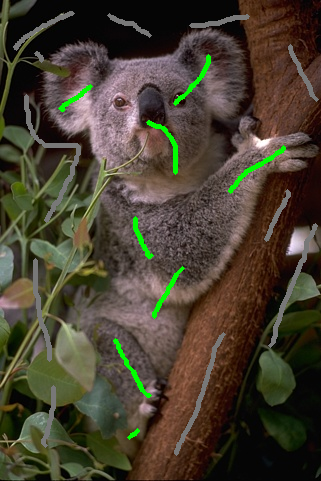
\includegraphics[scale=0.25]{images/segmentation/bc/coala/seeds.png} & 
	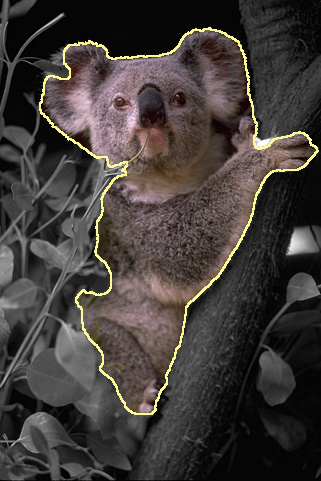
\includegraphics[scale=0.25]{images/segmentation/bc/coala/r3/lg0_sq05_dt1_it50.png} & 
	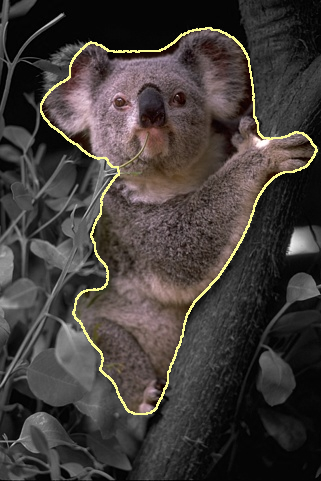
\includegraphics[scale=0.25]{images/segmentation/bc/coala/r3/lg0_sq1_dt1_it50.png} \\
	
 	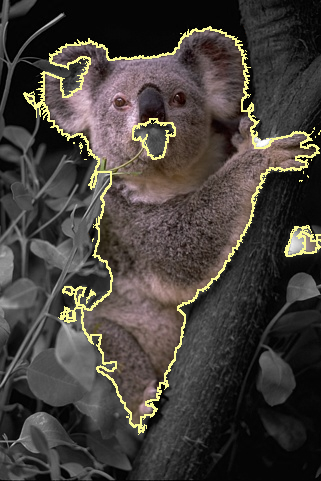
\includegraphics[scale=0.25]{images/segmentation/bc/coala/lg0_sq0_dt1_it20.png} & 
	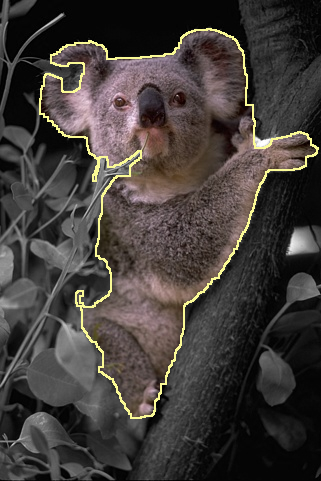
\includegraphics[scale=0.25]{images/segmentation/bc/coala/r3/lg1_sq0_dt1_it50.png} &
	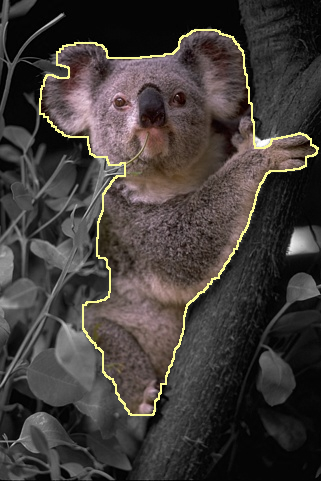
\includegraphics[scale=0.25]{images/segmentation/bc/coala/r3/lg2_sq0_dt1_it50.png} \\

	GrabCut & $(\alpha=0.5, \beta=0)$ & $(\alpha=1, \beta=0)$
\end{tabular}	
\caption{Comparison of squared curvature regularization (first row) and length regularization (second row). }
\label{fig:parameters-influence}
\end{figure}

\begin{figure}
	\center
	\begin{tabular}{ccc}
		GrabCut & Contour Correction & Schoenemann \\
		& $(r=5, \alpha=0.1, \beta=1.0, \gamma=3.0$) & $(\alpha=0.1, \beta=1.0$)\\
		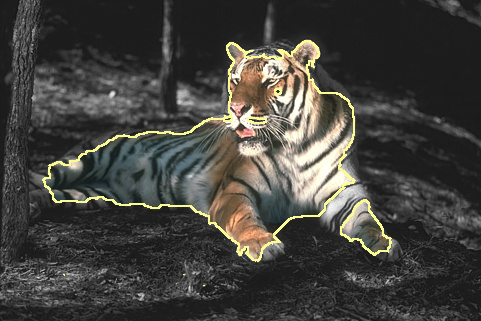
\includegraphics[scale=0.2]{images/segmentation/bc/tiger1/gc-seg.png} &
		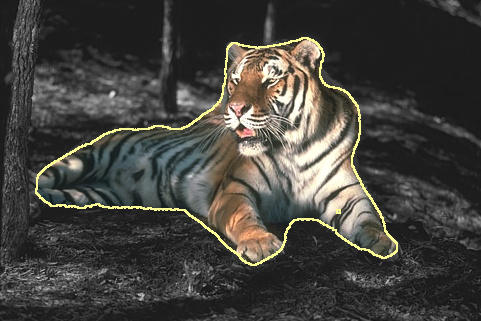
\includegraphics[scale=0.2]{images/segmentation/bc/tiger1/corrected-seg.png} &					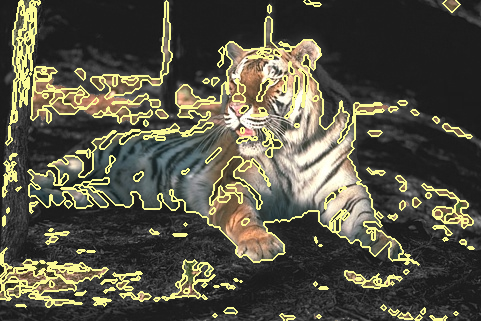
\includegraphics[scale=0.2]{images/segmentation/schoenemann/tiger1/tiger1-seg.png}\\									
		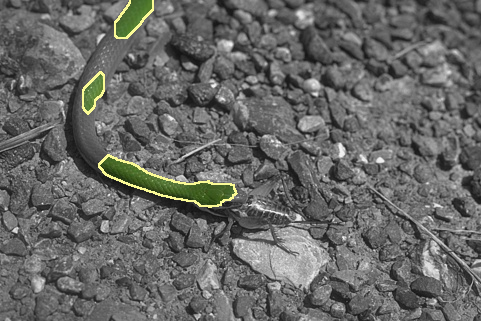
\includegraphics[scale=0.2]{images/segmentation/bc/snake/gc-seg.png} &
		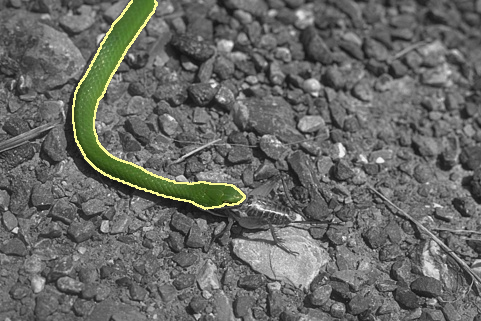
\includegraphics[scale=0.2]{images/segmentation/bc/snake/corrected-seg.png} &
		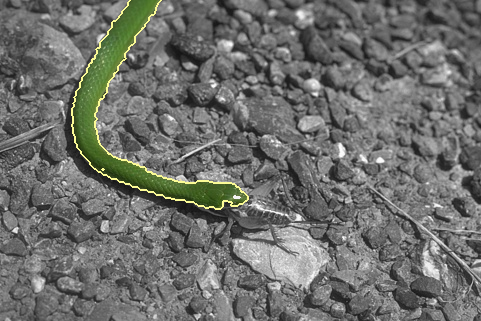
\includegraphics[scale=0.2]{images/segmentation/schoenemann/snake/snake-seg.png}\\						
		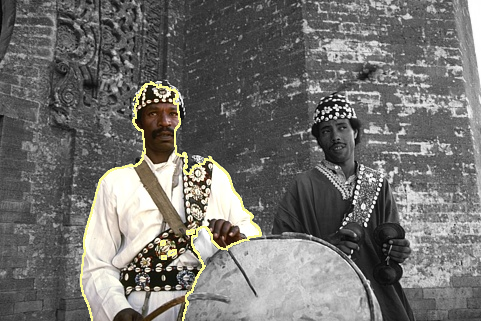
\includegraphics[scale=0.2]{images/segmentation/bc/man/gc-seg.png} &
		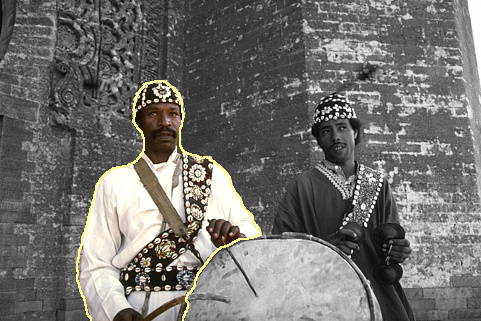
\includegraphics[scale=0.2]{images/segmentation/bc/man/corrected-seg.png} &
		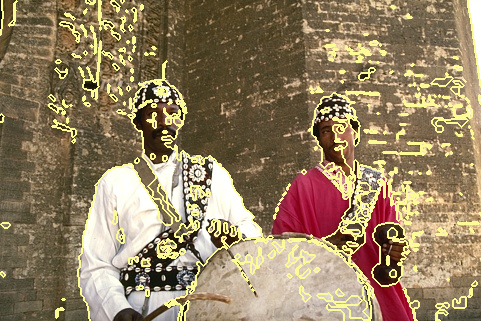
\includegraphics[scale=0.2]{images/segmentation/schoenemann/man/man-seg.png}\\		
		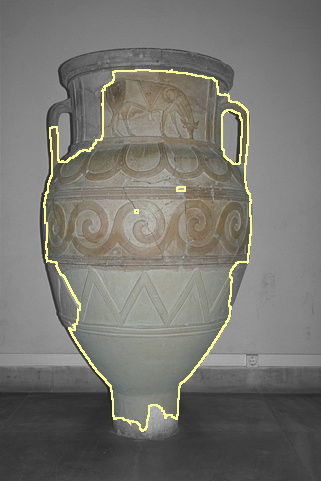
\includegraphics[scale=0.2]{images/segmentation/bc/vase/gc-seg.png} &
		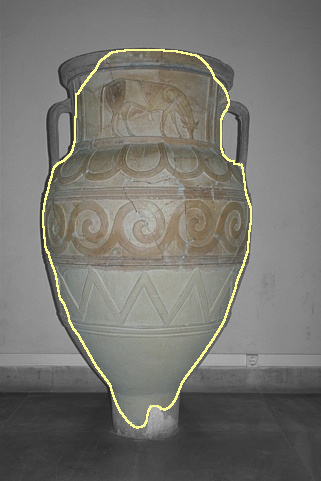
\includegraphics[scale=0.2]{images/segmentation/bc/vase/corrected-seg.png} &					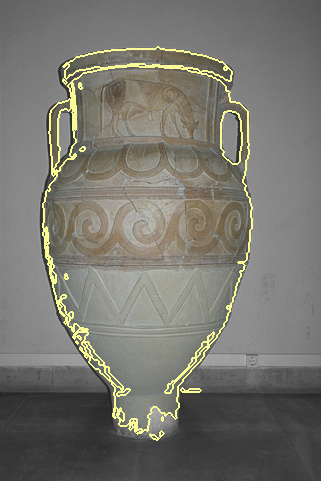
\includegraphics[scale=0.2]{images/segmentation/schoenemann/vase/vase-seg.png}		
	\end{tabular}
	\caption{The proposed method regularizes grabcut contours and returns meaningful results. We can observe the completion feature of curvature in the second row, and we don't suffer from oversegmentation issues as Schoenemann's method. However, our flow may stop in a local optima as in the fourth row, while Schoenemann's is able to extrapolate such solutions.}
	\label{fig:segmentation-results}	
\end{figure}


\begin{figure}
	\center
	\begin{tabular}{ccc}
		GrabCut & Contour Correction & Schoenemann \\
		& $(r=5, \alpha=0.1, \beta=1.0, \gamma=3.0$) & $(\alpha=0.1, \beta=1.0$)\\
		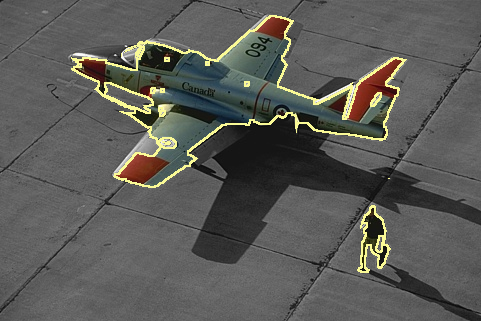
\includegraphics[scale=0.2]{images/segmentation/bc/airplane2/gc-seg.png} &
		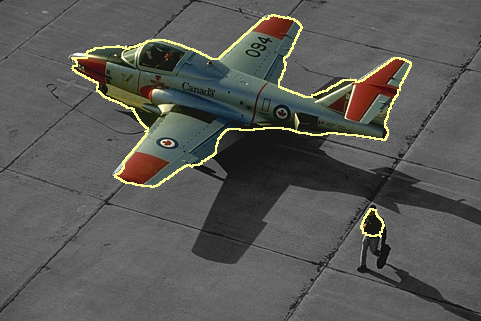
\includegraphics[scale=0.2]{images/segmentation/bc/airplane2/corrected-seg.png} &					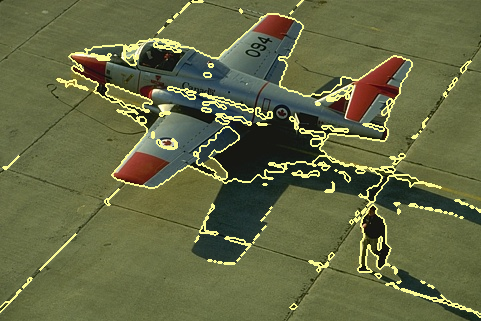
\includegraphics[scale=0.2]{images/segmentation/schoenemann/airplane2/airplane2-seg.png}\\									
		\includegraphics[scale=0.2]{images/segmentation/bc/bird/gc-seg.png} &
		\includegraphics[scale=0.2]{images/segmentation/bc/bird/corrected-seg.png} &
		\includegraphics[scale=0.2]{images/segmentation/schoenemann/bird/bird-seg.png}\\						
		\includegraphics[scale=0.2]{images/segmentation/bc/camel/gc-seg.png} &
		\includegraphics[scale=0.2]{images/segmentation/bc/camel/corrected-seg.png} &
		\includegraphics[scale=0.2]{images/segmentation/schoenemann/camel/camel-seg.png}\\		
		\includegraphics[scale=0.2]{images/segmentation/bc/rock/gc-seg.png} &
		\includegraphics[scale=0.2]{images/segmentation/bc/rock/corrected-seg.png} &					\includegraphics[scale=0.2]{images/segmentation/schoenemann/rock/rock-seg.png}\\
		\includegraphics[scale=0.2]{images/segmentation/bc/giraffes/gc-seg.png} &
		\includegraphics[scale=0.2]{images/segmentation/bc/giraffes/corrected-seg.png} &					\includegraphics[scale=0.2]{images/segmentation/schoenemann/giraffes/giraffes-seg.png}\\
		\includegraphics[scale=0.2]{images/segmentation/bc/canguru/gc-seg.png} &
		\includegraphics[scale=0.2]{images/segmentation/bc/canguru/corrected-seg.png} &					\includegraphics[scale=0.2]{images/segmentation/schoenemann/canguru/canguru-seg.png}\\		
		\includegraphics[scale=0.2]{images/segmentation/bc/coral/gc-seg.png} &
		\includegraphics[scale=0.2]{images/segmentation/bc/coral/corrected-seg.png} &					\includegraphics[scale=0.2]{images/segmentation/schoenemann/coral/coral-seg.png}\\				
						
	\end{tabular}
	\caption{}
	\label{fig:more-segmentation-results}	
\end{figure}


We evaluate our method using the BSD300 database \cite{martinFTM01berkeley}. All images contains the same number of pixels, the resolution being 321x481 in portrait mode. We compare the results of our method with segmentations given by GrabCut and Schoenemanns's method \cite{schoenemann09linear}. We report an average of $3s$ per flow iteration, and an average of $30$ iterations per image. While GrabCut executes in less than one second, Schoenemann's method may take $2$ hours to complete.


In figure \ref{fig:parameters-influence} we can observe the results of a curvature regularization in comparison with a pure length regularization, and figure \ref{fig:segmentation-results} shows some segmentation results.



\section{Conclusion}\label{sec:conclusion}


We've described two digital evolutions models based on the elastica energy and we've presented an application of one of them in image segmentation. The processes we've described are completely digital, and do not suffer from issues that typically arises in models that passes through a discretization stage, as rounding. Moreover, the model can handle changes in topology and its results are competitive with similar approaches while achieving a reasonable running time. 

Future developments of this work may include automatization, no more dependence on seeds selected by the user and automatic choice of radius based on the reach of the shape. One can also think to extend the model to the $3$d case, as the integral invariant estimator preserves its properties in that space. In the latter, a denoising application may be derived by running the flow on the $3$d shape defined by color and position.



%
% ---- Bibliography ----
%
% BibTeX users should specify bibliography style 'splncs04'.
% References will then be sorted and formatted in the correct style.
%
\bibliographystyle{splncs04}
\bibliography{jmiv}

\end{document}
